\documentclass[fancy, oneside, mastersfancy, ms]{byuthesis}
\usepackage{bookmark}


\usepackage{color}
\usepackage{fancyvrb}
\newcommand{\VerbBar}{|}
\newcommand{\VERB}{\Verb[commandchars=\\\{\}]}
\DefineVerbatimEnvironment{Highlighting}{Verbatim}{commandchars=\\\{\}}
% Add ',fontsize=\small' for more characters per line
\usepackage{framed}
\definecolor{shadecolor}{RGB}{241,243,245}
\newenvironment{Shaded}{\begin{snugshade}}{\end{snugshade}}
\newcommand{\AlertTok}[1]{\textcolor[rgb]{0.68,0.00,0.00}{#1}}
\newcommand{\AnnotationTok}[1]{\textcolor[rgb]{0.37,0.37,0.37}{#1}}
\newcommand{\AttributeTok}[1]{\textcolor[rgb]{0.40,0.45,0.13}{#1}}
\newcommand{\BaseNTok}[1]{\textcolor[rgb]{0.68,0.00,0.00}{#1}}
\newcommand{\BuiltInTok}[1]{\textcolor[rgb]{0.00,0.23,0.31}{#1}}
\newcommand{\CharTok}[1]{\textcolor[rgb]{0.13,0.47,0.30}{#1}}
\newcommand{\CommentTok}[1]{\textcolor[rgb]{0.37,0.37,0.37}{#1}}
\newcommand{\CommentVarTok}[1]{\textcolor[rgb]{0.37,0.37,0.37}{\textit{#1}}}
\newcommand{\ConstantTok}[1]{\textcolor[rgb]{0.56,0.35,0.01}{#1}}
\newcommand{\ControlFlowTok}[1]{\textcolor[rgb]{0.00,0.23,0.31}{#1}}
\newcommand{\DataTypeTok}[1]{\textcolor[rgb]{0.68,0.00,0.00}{#1}}
\newcommand{\DecValTok}[1]{\textcolor[rgb]{0.68,0.00,0.00}{#1}}
\newcommand{\DocumentationTok}[1]{\textcolor[rgb]{0.37,0.37,0.37}{\textit{#1}}}
\newcommand{\ErrorTok}[1]{\textcolor[rgb]{0.68,0.00,0.00}{#1}}
\newcommand{\ExtensionTok}[1]{\textcolor[rgb]{0.00,0.23,0.31}{#1}}
\newcommand{\FloatTok}[1]{\textcolor[rgb]{0.68,0.00,0.00}{#1}}
\newcommand{\FunctionTok}[1]{\textcolor[rgb]{0.28,0.35,0.67}{#1}}
\newcommand{\ImportTok}[1]{\textcolor[rgb]{0.00,0.46,0.62}{#1}}
\newcommand{\InformationTok}[1]{\textcolor[rgb]{0.37,0.37,0.37}{#1}}
\newcommand{\KeywordTok}[1]{\textcolor[rgb]{0.00,0.23,0.31}{#1}}
\newcommand{\NormalTok}[1]{\textcolor[rgb]{0.00,0.23,0.31}{#1}}
\newcommand{\OperatorTok}[1]{\textcolor[rgb]{0.37,0.37,0.37}{#1}}
\newcommand{\OtherTok}[1]{\textcolor[rgb]{0.00,0.23,0.31}{#1}}
\newcommand{\PreprocessorTok}[1]{\textcolor[rgb]{0.68,0.00,0.00}{#1}}
\newcommand{\RegionMarkerTok}[1]{\textcolor[rgb]{0.00,0.23,0.31}{#1}}
\newcommand{\SpecialCharTok}[1]{\textcolor[rgb]{0.37,0.37,0.37}{#1}}
\newcommand{\SpecialStringTok}[1]{\textcolor[rgb]{0.13,0.47,0.30}{#1}}
\newcommand{\StringTok}[1]{\textcolor[rgb]{0.13,0.47,0.30}{#1}}
\newcommand{\VariableTok}[1]{\textcolor[rgb]{0.07,0.07,0.07}{#1}}
\newcommand{\VerbatimStringTok}[1]{\textcolor[rgb]{0.13,0.47,0.30}{#1}}
\newcommand{\WarningTok}[1]{\textcolor[rgb]{0.37,0.37,0.37}{\textit{#1}}}

\providecommand{\tightlist}{%
  \setlength{\itemsep}{0pt}\setlength{\parskip}{0pt}}\usepackage{longtable,booktabs,array}
\usepackage{calc} % for calculating minipage widths
% Correct order of tables after \paragraph or \subparagraph
\usepackage{etoolbox}
\makeatletter
\patchcmd\longtable{\par}{\if@noskipsec\mbox{}\fi\par}{}{}
\makeatother
% Allow footnotes in longtable head/foot
\IfFileExists{footnotehyper.sty}{\usepackage{footnotehyper}}{\usepackage{footnote}}
\makesavenoteenv{longtable}
\usepackage{graphicx}
\makeatletter
\def\maxwidth{\ifdim\Gin@nat@width>\linewidth\linewidth\else\Gin@nat@width\fi}
\def\maxheight{\ifdim\Gin@nat@height>\textheight\textheight\else\Gin@nat@height\fi}
\makeatother
% Scale images if necessary, so that they will not overflow the page
% margins by default, and it is still possible to overwrite the defaults
% using explicit options in \includegraphics[width, height, ...]{}
\setkeys{Gin}{width=\maxwidth,height=\maxheight,keepaspectratio}
% Set default figure placement to htbp
\makeatletter
\def\fps@figure{htbp}
\makeatother
\newlength{\cslhangindent}
\setlength{\cslhangindent}{1.5em}
\newlength{\csllabelwidth}
\setlength{\csllabelwidth}{3em}
\newlength{\cslentryspacingunit} % times entry-spacing
\setlength{\cslentryspacingunit}{\parskip}
\newenvironment{CSLReferences}[2] % #1 hanging-ident, #2 entry spacing
 {% don't indent paragraphs
  \setlength{\parindent}{0pt}
  % turn on hanging indent if param 1 is 1
  \ifodd #1
  \let\oldpar\par
  \def\par{\hangindent=\cslhangindent\oldpar}
  \fi
  % set entry spacing
  \setlength{\parskip}{#2\cslentryspacingunit}
 }%
 {}
\usepackage{calc}
\newcommand{\CSLBlock}[1]{#1\hfill\break}
\newcommand{\CSLLeftMargin}[1]{\parbox[t]{\csllabelwidth}{#1}}
\newcommand{\CSLRightInline}[1]{\parbox[t]{\linewidth - \csllabelwidth}{#1}\break}
\newcommand{\CSLIndent}[1]{\hspace{\cslhangindent}#1}

\usepackage{booktabs}
\usepackage{longtable}
\usepackage{array}
\usepackage{multirow}
\usepackage{wrapfig}
\usepackage{float}
\usepackage{colortbl}
\usepackage{pdflscape}
\usepackage{tabu}
\usepackage{threeparttable}
\usepackage{threeparttablex}
\usepackage[normalem]{ulem}
\usepackage{makecell}
\usepackage{xcolor}
\usepackage{siunitx}
\usepackage{booktabs}
\usepackage{longtable}
\usepackage{array}
\usepackage{multirow}
\usepackage{wrapfig}
\usepackage{float}
\usepackage{colortbl}
\usepackage{pdflscape}
\usepackage{tabu}
\usepackage{threeparttable}
\usepackage{threeparttablex}
\usepackage[normalem]{ulem}
\usepackage[utf8]{inputenc}
\usepackage{makecell}
\usepackage{xcolor}
\makeatletter
\makeatother
\makeatletter
\@ifpackageloaded{bookmark}{}{\usepackage{bookmark}}
\makeatother
\makeatletter
\@ifpackageloaded{caption}{}{\usepackage{caption}}
\AtBeginDocument{%
\ifdefined\contentsname
  \renewcommand*\contentsname{Table of contents}
\else
  \newcommand\contentsname{Table of contents}
\fi
\ifdefined\listfigurename
  \renewcommand*\listfigurename{List of Figures}
\else
  \newcommand\listfigurename{List of Figures}
\fi
\ifdefined\listtablename
  \renewcommand*\listtablename{List of Tables}
\else
  \newcommand\listtablename{List of Tables}
\fi
\ifdefined\figurename
  \renewcommand*\figurename{Figure}
\else
  \newcommand\figurename{Figure}
\fi
\ifdefined\tablename
  \renewcommand*\tablename{Table}
\else
  \newcommand\tablename{Table}
\fi
}
\@ifpackageloaded{float}{}{\usepackage{float}}
\floatstyle{ruled}
\@ifundefined{c@chapter}{\newfloat{codelisting}{h}{lop}}{\newfloat{codelisting}{h}{lop}[chapter]}
\floatname{codelisting}{Listing}
\newcommand*\listoflistings{\listof{codelisting}{List of Listings}}
\makeatother
\makeatletter
\@ifpackageloaded{caption}{}{\usepackage{caption}}
\@ifpackageloaded{subcaption}{}{\usepackage{subcaption}}
\makeatother
\makeatletter
\@ifpackageloaded{tcolorbox}{}{\usepackage[skins,breakable]{tcolorbox}}
\makeatother
\makeatletter
\@ifundefined{shadecolor}{\definecolor{shadecolor}{rgb}{.97, .97, .97}}
\makeatother
\makeatletter
\makeatother
\makeatletter
\makeatother

\title{Simulating Incident Management Team Response and Performance}
\author{Daniel Jarvis}

% On the custom title page, use the same title, but format as you like
\customtitle{Simulating Incident Management Team Response and
Performance}

% This is the date of graduation
\date{2023-06-25}

% If your degree is not a PhD or MS, then you can overwrite the degree using 
% the \degree command: \degree{Bachelors of Basics}

% Your department
\department{Civil and Construction Engineering}

% The names of your committee members
\committeechair{Gregory S. Macfarlane}
  \committeemember{Grant G. Schultz}
  \committeemember{Gustavious P. Williams}

\keywords{
    Incident Management Teams; Incident Simulation;  
    Transportation Modeling
}

\begin{document}

\frontmatter
\titlepage
\cleardoublepage

\customtitlepage
\cleardoublepage


  \begin{abstract}
The effectiveness of Incident Management Teams (IMT) in reducing the
duration and impact of traffic incidents is well-documented. The
capacity of large-scale simulation models to illustrate the negative
effects of these incidents on vehicle delays and excess user costs (EUC)
is also widely recognized. However, there is a gap in research
integrating large-scale simulation modeling with IMT performance
analysis. This study uses the Multi Agent Transport Simulation (MATSim)
framework to simulate the impact of incidents and evaluate the
performance of IMT across the regional network of Utah's Wasatch Front,
analyzing their operation in various hypothetical situations.

Our findings validate the role of IMT in decreasing delays and EUC. The
simulation also investigates the potential effects of increased incident
frequency and IMT expansion, revealing that more incidents increased
delays, whereas additional IMT units can mitigate these effects and
improve response times.

The MATSim model we developed demonstrates the potential of dynamic
large-scale modeling to evaluate incident management strategies in ways
that previous studies did not. This model could serve as a valuable tool
for further evaluating the performance of Utah's IMT program, with the
potential to offer new perspectives on optimizing team deployment and
scheduling efficiency.
\end{abstract}
\cleardoublepage

\begin{acknowledgments}
I want to extend my gratitude to the Utah Department of Transportation
for their substantial financial backing, which was essential for the
completion of my research and thesis project. I am equally grateful to
the technical advisory committee, whose expert guidance and invaluable
feedback were essential throughout my research endeavor. Their in-depth
understanding of Utah's traffic incident management programs was a
crucial contributor to the successful outcome of this study.

My sincere thanks are extended to my fellow research assistants at
BYU---Joel Hyer, Harrison Holdsworth, and Brynn Woolley. Joel's
insightful analysis and the vital data he provided from the IMT
Performance Phase III project were indispensable. Harrison's
wide-ranging input, from his diligent compilation of research on IMT
optimization to his collaborative efforts in drafting the literature
review, proved instrumental. His ability to seamlessly connect Joel's
work with my research was invaluable. Brynn's expertise in developing
the transportation model, her astute analysis of its findings, and her
assistance in refining and editing this report added significantly to
the quality of my work.

Profound appreciation is due to my faculty advisors and the members of
my thesis committee, Drs. Macfarlane, Schultz, and Williams, for their
unwavering support. I am particularly indebted to Dr.~Macfarlane for his
exceptional mentorship as an advisor, educator, and friend. His
patience, wisdom, and encouragement have been instrumental at every
stage of my academic journey. His faith in me and consistent support
have been the pillars of my personal development and the achievements of
this research.

Lastly, I offer thanks to my parents, Duane and Jodi Jarvis, for their
steadfast encouragement and belief in me throughout my academic
pursuits. Their encouragement and reassurance have been a source of
immense strength, especially during this significant stage of my life. I
am forever grateful for the stability and unwavering support they have
so selflessly provided.
\end{acknowledgments}
\cleardoublepage

	\tableofcontents*
	\cleardoublepage

	\listoffigures
	\cleardoublepage

	\listoftables
	\cleardoublepage

\mainmatter
\bookmarksetup{startatroot}

\hypertarget{introduction}{%
\chapter{Introduction}\label{introduction}}

\footnote{This is a draft of a manuscript, authored by Jarvis,
  Macfarlane, Woolley, and Schultz. It is prepared to be submitted to
  the Transportation Research Part C. Any use of the pronoun `we' in
  this document refers collectively to the research team, all of whom
  will be listed as authors upon the manuscript's publication as an
  article.} Incident Management Teams (IMTs) are service vehicles that
collaborate with highway patrol units to manage traffic after an
incident and provide timely roadside assistance. They are strategically
important for improving highway operations, particularly during peak
traffic times, helping to effectively alleviate congestion and
associated user costs. Capable of quickly addressing a range of
incidents from minor vehicle breakdowns to severe multi-car collisions,
IMTs are crucial in controlling traffic and restoring normal flow on the
roadways.

States like Utah have long benefited from IMT programs, witnessing
notable reductions in congestion and traffic-related costs (Bennett et
al., 2022). The effectiveness of IMTs, influenced by factors such as
response times (Bennett et al., 2021), fleet size (Kim et al., 2012),
and deployment locations (Ozbay et al., 2013), is well-documented.
However, the current understanding primarily stems from ad-hoc models
and independent initiatives, leaving a gap in regional-scale traffic
delay modeling associated with incident management.

A study by Kaddoura \& Nagel (2018) highlights the efficacy of
large-scale traffic models in evaluating regional incident impacts,
showing increases in congestion and travel times in a simulated network.
However, it doesn't assess the effects of IMT strategies. Our research
aims to fill this gap by integrating IMT data into a large-scale
regional traffic model, focusing on the impacts of traffic incidents and
IMT interventions within such a simulated network.

In this research, we present a model of IMT responses to incidents on
freeways in the Wasatch Front region of Utah. The model uses the Multi
Agent Transportation Simulation (MATSim) framework to evaluate IMT
effectiveness within various traffic incident scenarios. After
conducting 60 simulations, we compared their outcomes and evaluated the
effectiveness of IMTs at improving traffic conditions and reducing
congestion.

The paper proceeds in a typical order.
\protect\hyperlink{sec-literature}{The literature review} contains a
discussion of previous research into IMT effectiveness and optimization.
The \protect\hyperlink{sec-methods}{methodology section} describes the
simulation and scenario construction, while
\protect\hyperlink{sec-results}{the results} present the findings of the
analysis alongside a discussion of their implications. The paper's
\protect\hyperlink{sec-conclusions}{conclusions} provide an outline of
future research motivated by this study's limitations.

\bookmarksetup{startatroot}

\hypertarget{sec-literature}{%
\chapter{Literature Review}\label{sec-literature}}

Traffic incident management in general---and IMTs in particular --- are
not strictly new innovations. The Federal Highway Administration (FHWA)
publishes the \emph{Traffic Incident Management Handbook} (Owens et al.,
2010), which defines traffic incident management as:

\begin{quote}
\emph{The systematic, planned, and coordinated use of human,
institutional, mechanical, and technical resources to reduce the
duration and impact of incidents and improve the safety of motorists,
crash victims, and incident responders (Owens et al., 2010, pp. 1--1).}
\end{quote}

\noindent The handbook details the process of how to implement a traffic
incident management program as well as improve it. The manual covers
various aspects of incident management, including the responsibilities
of emergency medical teams, law enforcement, and other responding
entities. For this research, we focus on the dedicated traffic incident
management teams operated by departments of transportation or similar
agencies and not on other types of first responders.

FHWA has established performance measures to develop a framework to
quantify improvements to IMT operations (Owens et al., 2010). A specific
measure related to this research is roadway clearance time (RCT): the
time between the first recordable awareness of the incident and the time
all lanes open for traffic flow. Numerous studies have assessed the
impact of Traffic Incident Management programs on traffic conditions,
utilizing the performance measures provided by FHWA. A particularly
noteworthy study conducted by Hadfield et al. (2021) explores the
relationship between IMT response time (RT) and RCT. This research
leveraged interconnected data from the Utah Department of Transportation
(UDOT) and the Utah Highway Patrol (UHP), aiming to quantify the traffic
improvements resulting from swift IMT interventions at incident sites.
Analyzing 63 incidents, the study found that a one-minute delay in IMT
response correlated with a 0.8-minute increase in RCT. This delay also
impacted an additional 93 vehicles, added roughly 34.6 minutes to the
network's total estimated travel time, and resulted in an extra \$925 in
excess user costs (EUC). Hadfield et al. (2021) established a clear
connection between timely IMT responses and improved traffic conditions,
highlighting the importance of rapid intervention.

Skabardonis (1998) confirmed the effectiveness of IMTs in their study,
concluding that IMTs in California effectively reduced incident RT and
EUC. Skabardonis (1998) found that, on average, total incident RT was 15
minutes longer when California Highway Patrol responded without the
support of IMTs. Using a system to assign a cost per traveler per unit
of time to vehicles in the observed area, the authors determined that
IMT units had a cost-to-benefit ratio of 5:1. They also concluded that
patrol officers spent less time on incidents (including vehicle
breakdowns) when assisted by IMT services.

\hypertarget{sec-lit_imt_opt}{%
\section{IMT Optimization}\label{sec-lit_imt_opt}}

Given the evidence that IMT programs improve traffic conditions and
reduce costs for government entities and individuals, it becomes crucial
to further research avenues to maximize these benefits. One possible
strategy is the strategic placement of IMT units, optimizing their
spatial effectiveness to enhance their impact. Enhancing IMT programs
often focuses on the precise deployment of individual units and the
strategic positioning of IMT depots---locations where inactive teams
await dispatch. For scenarios where IMT vehicles are actively on patrol,
research often concerns designing an efficient service area. Various
methodologies have been applied to tackle this allocation challenge.
While some studies employ statistical models, incorporating a range of
variables to maximize specific performance measures, others opt for
digital modeling as a solution.

For instance, Ozbay et al. (2013) designed a mixed-integer programming
model with probabilistic constraints to optimize the allocation of IMTs
across ``depots'' or staging areas in New Jersey. This innovative
approach, grounded in known probabilities of various incident types,
strategically positions IMT units to respond to incidents, taking into
account future probabilities on the network. The primary goals were to
minimize incident management costs and maximize the likelihood that
every incident receive assistance. The model was applied to a simplified
New Jersey highway network, utilizing traffic incident data from the
region to inform demand distribution. Through this application, an
optimal number of depots and IMT assignments were determined. However,
the lack of a comparative analysis with pre-existing depot and unit
distributions meant that the exact improvements yielded by the model
remained unquantified.

Where Ozbay et al. (2013) focused on optimizing the IMT allocation in
specific zones, others have researched their effectiveness as roaming
entities. Lou et al. (2011) developed a mixed-integer nonlinear
optimization model and proposed different algorithms to minimize the RT
of IMTs. They modeled IMTs within specific freeway sections, and
incident frequencies were generated randomly on the network, given the
mean and standard deviations of incident occurrence on each link in the
network. The study focused on developing and optimizing these algorithms
for broad implementation rather than focusing on any particular network
or reducing response times in specific areas. They implemented a
template Sioux Falls network into the model as a practical
demonstration. Compared to the existing deployment plan in Sioux Falls,
the algorithm-generated plans could potentially reduce total RT by
16.5-20.8\%.

Each of the studies mentioned attempts to understand optimal IMT
deployment based on ad-hoc models, specially constructed utility
functions, or similar stand-alone efforts. While their results provide
valuable insights, they might be limited in their scope, as they do not
explicitly attempt to model the traffic delay associated with incident
management at a large scale. Research modeling the effects of incidents
on region-scale traffic networks is a recent innovation, providing a
more holistic view of their impact. This approach is potentially
beneficial for comprehensively assessing the effectiveness of IMT and
paves the way for our subsequent discussion in
\protect\hyperlink{sec-inc_modeling}{incident modeling}, where we will
discuss the advancements and applications of this innovative research
domain.

\hypertarget{sec-inc_modeling}{%
\section{Incident Modeling}\label{sec-inc_modeling}}

The majority of traffic models used to study the impacts of incidents
and incident management are Dynamic Traffic Assignment (DTA) models.
These models demonstrate how congestion and travel times fluctuate over
time, varying for different vehicles (Chiu et al., 2011). The capability
to represent travel time variance make DTA models particularly
advantageous for depicting the unpredictability of incidents. A study
conducted by Sisiopiku et al. (2007), which explored the effects of
congestion, underscored the applications of simulation-based DTA
modeling in incident management. It advocated for dynamic assignment as
the optimal approach for incident modeling. Sisiopiku et al. (2007)
describes their methodology as follows:

\begin{quote}
\emph{The overall approach in this study is to use the DTA capabilities
to support decision-making for incident management. DTA is particularly
appropriate for studying short-term planning applications such as
evaluating various incident management options (Sisiopiku et al., 2007,
p. 111).}
\end{quote}

In their study, Sisiopiku et al. (2007) employed a DTA model to
understand the impacts of diverse incident scenarios and to assess the
effectiveness of potential incident management strategies and traffic
control methods. The research commenced with a baseline scenario under
standard conditions, establishing a reference point for evaluating
incident impacts. Subsequent scenarios simulated incidents without
notifying drivers, with variations in the duration and severity of the
incidents. The final scenario replicated the previous one but
incorporated information provision to drivers, enabling them to optimize
their routes and access preplanned diversion paths, with guidance from
Variable Message Signs. Conducted in Birmingham and Chicago, the study
illustrated that post-incident information provision could result in
travel time savings and reduced traffic delays, highlighting the DTA
model's utility in simulating the effects of incidents and evaluating
traffic management and control strategies.

The Sisiopiku et al. (2007) study used the Visual Interactive System for
Transport Algorithms (VISTA) as their specific modeling tool. Despite
its efficacy, VISTA was critiqued by Wirtz et al. (2005) for its
inherent assumption that all drivers have perfect travel time
information for routing to the optimal path. For example, the Sisiopiku
et al. (2007) study assumed a 100\% compliance rate with the provided
diversion routes in their model. However, the research by Wirtz et al.
(2005) revealed that ``less-informed drivers spend more time traveling
than necessary, representing a departure from the user-optimal traffic
conditions simulated by VISTA.'' (Wirtz et al., 2005) This critique does
not invalidate the findings of Sisiopiku et al. (2007) but highlights
the limitations of VISTA in reflecting real-world travel behavior.

VISTA is categorized as a large-scale, or mesoscopic, model suitable for
modeling extensive networks. Conversely, small-scale, or microscopic,
models, capable of tracking precise vehicle locations, driver behavior,
and vehicle characteristics, offer a highly realistic representation but
are impractical for large regions (Chiu et al., 2011). In Australia, Dia
\& Cottman (2006) used a simulation model, VISSIM, to assess the impacts
of incident management on two arterial routes connecting the western
suburbs of Brisbane to the Central Business District. Although VISSIM is
a primary traffic modeling tool for UDOT, its detailed precision renders
it impractical for modeling incidents and IMT impacts along the Wasatch
Front. Given this research's scope, a large-scale dynamic model would
likely be the most suitable choice.

Interestingly, Pal \& Sinha (2002) developed a model to replicate the
impacts of incidents and IMTs on traffic conditions in Indiana utilizing
overall traffic conditions as the performance indicator for IMT
effectiveness. Various configurations of response vehicles were
simulated, incorporating probability distributions of crash data,
vehicle speed, and roadway carrying capacity. The study's results
informed recommendations on fleet size, operation hours, patrol area
design, and dispatching policy improvements. However, since mesoscopic
traffic simulations in 2002 could not simulate incident response units,
Pal \& Sinha (2002) had to create their model from scratch.
Unfortunately, their model and methodology seem tailored specifically
for their study and may not be applicable to this project's context.

Similar to VISTA, MATSim, the Multi Agent Transport Simulation toolkit,
stands as another large-scale modeling system that has proven effective
in conducting large-scale incident simulations. While VISTA and MATSim
both have the capability to simulate the regional impact of traffic
incidents, MATSim presents attributes that could potentially offer a
more accurate representation of real-world scenarios and driver
behaviors. Also, contrary to the model crafted by Pal \& Sinha (2002),
MATSim operates as an open-source framework, making it ideal for
adapting to different scenarios. Notably, MATSim facilitates the
integration of real world data, enhancing the authenticity and precision
of network simulations. This capability is particularly pertinent to
this project, as prior research conducted by Schultz et al. (2023) has
made recent UDOT incident and IMT data available, which could be
integrated into the simulation model for more robust and realistic
results. Although MATSim has been employed to assess network impacts of
incidents, its application in incident management studies remains
largely unexplored, presenting an opportunity for further investigation
and potential breakthroughs in the field.

Kaddoura \& Nagel (2018) conducted a comprehensive study on incident
modeling using MATSim, representing transport users as individual agents
within an iterative framework that allows for adjustments to travel
plans both within and between iterations. They accessed incident data,
including Traffic Message Channel (TMC) information detailing cause and
severity, via the HERE application programming interface. This rich
dataset enabled the classification of incidents as either long-term,
such as multiple-day lane closures, or short-term, affecting transport
supply for less than a day. Applying their model to an inner-city
network in Berlin, Germany, Figure \ref{fig-berlin-cap} illustrates the
modeled incident severities.

\begin{figure}
\centering
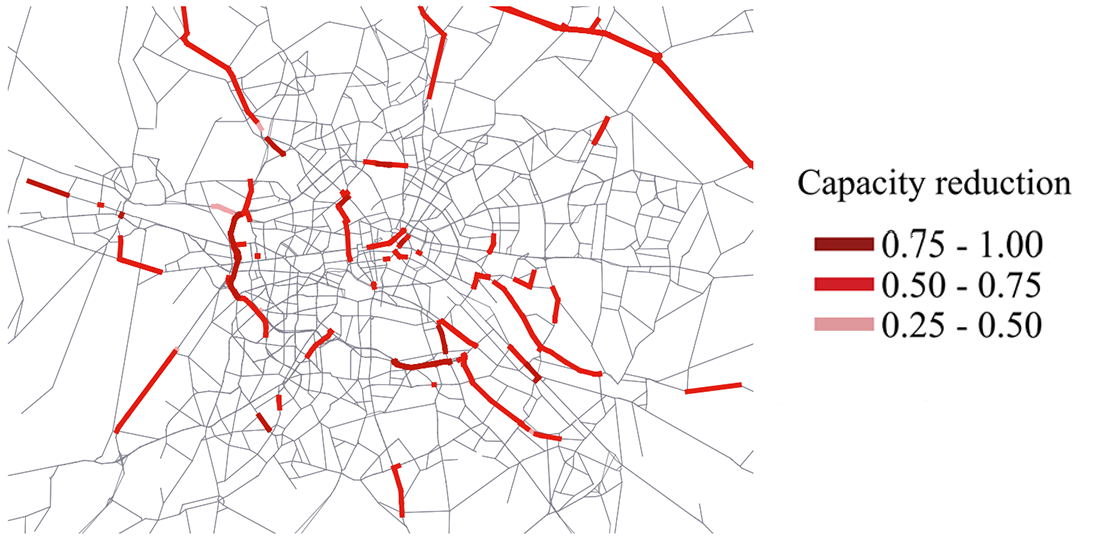
\includegraphics{figures/berlin_capacity.png}
\caption[Traffic incidents mapped on the Berlin network.]{Traffic incidents mapped on the Berlin network (Kaddoura \& Nagel, 2018).}
\label{fig-berlin-cap}
\end{figure}

Kaddoura \& Nagel (2018) found that long-term traffic incidents increase
traffic congestion and the average car travel time by 313 sec (+18\%)
per trip. Short-term traffic incidents increase the average travel time
per car trip by another 136 sec (+8\%). Additionally, they found that
for 44\% of all car trips, the agent's transport route contained at
least one road segment for which the capacity or speed limit was reduced
because of an incident. Their study concluded that networks in which
transport users had high levels of knowledge about the incidents and
resulting traffic congestion still experienced an increase in travel
time caused by long and short-term incidents. Finally, the authors
asserted that ``accounting for traffic incidents makes the model more
realistic, allowing for an improved policy investigation'' (Kaddoura \&
Nagel, 2018, p. 885). The modeling performed by Kaddoura \& Nagel (2018)
is just one example of research on MATSim's capacity for incident-based
simulations.

A MATSim incidents model developed by Li \& Ferguson (2020) included
various rescheduling options, such as departure time, mode choice, and
trip cancellation. Their simulation found that if travelers received
notice of an incident, they would either depart early from their place
of origin or switch to public transport (Li \& Ferguson, 2020). The
process proposed by Li and Ferguson is beneficial because it allows
agents to reassess their mode choice or route assignment based on the
notice of a reported incident. Li and Ferguson show that users care
about total travel time and travel time variability (risk tolerance to a
certain degree). Receiving notifications about incidents by agents
impacted both travel time and mode choice. They concluded that ``the
provision of real-time traffic information is a useful approach to
mitigating the side-effects of incidents through helping transport users
efficiently adapt their day plans'' (Li \& Ferguson, 2020, p. 96).
Additionally, they found that ``most of the travelers notified of being
affected by incidents are simulated to depart early or switch to public
transport, which effectively reduces the average travel time delay
caused by disruptions'' (Li \& Ferguson, 2020, p. 96). Their findings
validate the conclusions of Sisiopiku et al. (2007) that making incident
information available to agents leads to decreases in travel time and
congestion.

This subsection highlights the capabilities of DTA models to simulate
the complexities of traffic incidents, congestion, and travel times. It
highlights how incorporating incident management responses into the
models would enhance their ability to simulate realistic traffic
conditions and support policy analysis. Given its capacity to model
large-scale networks, integrate real-world data, and replicate realistic
driver behavior, MATSim is deemed particularly suitable for this
project.

\hypertarget{sec-lit_summary}{%
\section{Summary}\label{sec-lit_summary}}

This \protect\hyperlink{sec-literature}{literature review} summarizes
extensive research on IMTs role in reducing RCT and EUC during incidents
and optimizing their size and distribution. However, it reveals a gap:
these performance studies do not explore the broader impact of incidents
and IMT responses on large-scale networks. Similarly, while DTA modeling
studies assess incident impacts on network dynamics and driver behavior,
they seldom consider IMT influence. This gap limits understanding of
IMTs' effectiveness in congested networks. Our research aims to
integrate these areas, modeling incident response within a simulation to
evaluate IMT deployment strategies and effectiveness more
comprehensively.

\bookmarksetup{startatroot}

\hypertarget{sec-methods}{%
\chapter{Methodology}\label{sec-methods}}

As highlighted in the \protect\hyperlink{sec-literature}{literature
review}, there is substantial evidence indicating that IMTs can
effectively reduce RCT and EUC following traffic incidents.
Additionally, the effectiveness of DTA models in analyzing the impact of
such incidents has been well-documented. However, there is a lack of
comprehensive research evaluating IMTs impact on entire traffic networks
and their associated agents. To address this gap, it is necessary that
we develop a model capable of simulating both traffic incidents and the
ensuing IMT interventions, with the objective of gauging the efficiency
of IMT deployments. Due to its proficiency in regional-scale incident
simulation and its authentic portrayal of driver behavior, MATSim has
been identified as the most suitable model for this research. This
section describes the methodology, expounding on the model's
capabilities, the requisite data inputs, and the benchmarks established
for determining IMT effectiveness.

Our methodology is structured around three main components: the
functionality of the MATSim model, the setup of IMT vehicles and
incidents, and the scenarios for comparative analysis. In the
\protect\hyperlink{sec-MATSim_mod}{model design} subsection we describe
the structure of the model and the functions it uses to represent
incidents and IMT response. In \protect\hyperlink{sec-model_imp}{model
implementation} subsection we outline the data structure of the model by
describing the \protect\hyperlink{sec-IMT_setup}{setup of IMTs} and
explaining our \protect\hyperlink{sec-inc_data}{incident data and
sampling} methods. We conclude by describing the
\protect\hyperlink{sec-scenarios}{scenarios} we used for evaluating the
impact of incidents and IMTs.

\hypertarget{sec-MATSim_mod}{%
\section{Model Design}\label{sec-MATSim_mod}}

MATSim is an open-source framework used for conducting extensive,
agent-based transportation simulations on a large scale. Operating as a
dynamic traffic simulation, it is often used in demand modeling and
agent-based mobility analysis (Dobler et al., 2012). Thanks to its
open-source architecture, MATSim enables the seamless integration of a
diverse array of modules and packages into its models. Users across the
platform can create, import, and modify these components, fostering a
collaborative and innovative environment.

For the purposes of our research, we developed the ImtModule, a
specialized MATSim extension designed to process incidents and IMT
responses within the simulation. This module leverages existing research
on incident simulation, Demand Rapid Transit (DRT), event handling, and
vehicle dispatch algorithms, building upon these foundations to enhance
the functionality of our model.

In this section, we describe some of the specific tools within MATSim
that we used and adapted to construct a comprehensive and functional
model. These tools include \protect\hyperlink{sec-MATSim_score}{scoring
and replanning}, \protect\hyperlink{sec-NCE}{network change events}, and
\protect\hyperlink{sec-imt_response}{IMT assignment}. Together, they
contribute to the authenticity and precision of our traffic simulations,
particularly in the context of responding to roadway incidents, ensuring
that our model provides accurate and reliable results.

\hypertarget{sec-MATSim_Score}{%
\subsection{Scoring and Replanning}\label{sec-MATSim_Score}}

In MATSim, each individual within the simulation is called an agent.
These agents follow daily schedules, partaking in various activities and
modes of travel. Their actions are evaluated using a point system, which
takes into account the specifics of their travel, as highlighted by
Nagel et al. (2016). Timely arrivals at destinations are rewarded with
positive points, whereas delays result in deductions. Furthermore,
different transportation modes are assigned utility scores, which play a
crucial role in shaping the agents' travel preferences and decisions.

Each agent possesses a memory that stores plans from a certain number of
iterations, as well as replanning strategies that dictate how agents can
adjust their plans from iteration to iteration (Horni \& Nagel, 2016).
The size of an agent's memory is typically dependent on the size of the
model being run. In the case of our large-scale Utah model, we opted to
limit the agents' plan memory to just five iterations. The replanning
strategies used include selecting the plan with the highest score 80\%
of the time, opting to reroute 10\% of the time, and adjusting activity
timings for the remaining 10\%. Our selection for the remaining scoring
and replanning parameters drew from the incident research conducted by
Kaddoura \& Nagel (2018).

As will be detailed in the \protect\hyperlink{sec-model_imp}{model
implementation} subsection, the plans file used to generate simulations
in MATSim was exceptionally large, encompassing travel data for over 2
million agents. Our objective, utilizing the complete plans file, was to
guide the simulated agents toward an equilibrium in travel behavior. To
achieve this, we employed the following methodology:

\begin{enumerate}
\def\labelenumi{\arabic{enumi}.}
\tightlist
\item
  We processed both the network and plans files over the course of 350
  simulated iterations without any incidents or IMTs included.
\item
  Using the output from this preliminary scenario, we established a `hot
  start' for the subsequent scenarios incorporating incidents and IMT
  responses. At this stage, a significant portion of agents had already
  identified efficient travel routes to their destinations. This
  preliminary phase of running the plans file was intended to expedite
  the convergence towards a balanced state in travel behavior for
  scenarios that included incidents and IMT responses.
\item
  To achieve equilibrium in travel behavior, we conducted an additional
  100 iterations in the simulations that accounted for incidents and IMT
  responses, ensuring a more comprehensive stabilization across the
  majority of scenarios.
\end{enumerate}

Figure~\ref{fig-score-output} presents a MATSim scoring output from a
scenario incorporating incidents and IMT responses. The figure indicates
notable plan adjustments and corresponding score changes during the
first 60 iterations. As the simulation progressed, the executed scores
started to stabilize. To minimize the potential for significant
variance, replanning was disabled after the 85th iteration. This
approach ensures that the final iterations, which are critical for
scenario analysis, reflect a steady state.

\begin{figure}

{\centering \includegraphics{03_methods_files/figure-pdf/fig-score-output-1.pdf}

}

\caption{\label{fig-score-output}MATSim scoring statistics output
example.}

\end{figure}

\hypertarget{sec-NCE}{%
\subsection{Network Change Events}\label{sec-NCE}}

Within a MATSim network, each link is characterized by specific
attributes such as type, length, number of lanes, free-flow speed, and
capacity. To effectively simulate unexpected events and their subsequent
impacts on traffic flow, it is essential to dynamically adjust these
attributes. This capability, termed a Time-Dependent Network, is
explained in the MATSim textbook (Rieser et al., 2016) and is vital for
ensuring the realism and accuracy of our simulation.

Network Change Events (NCEs) serve as the mechanism within MATSim for
modifying network attributes at precise moments during a simulation.
Detailed in Section 6.1 of the MATSim textbook (Rieser et al., 2016),
the implementation of NCEs requires specific adjustments to the MATSim
configuration file to facilitate a time-variant network. These events
can modify a link's free-flow speed, number of lanes, or capacity. To
initiate an NCE, the system requires specific information including the
time of the event \texttt{startTime}, the affected link(s)
\texttt{link\ refID}, the type of change \texttt{free-flow\ speed},
\texttt{lanes}, or \texttt{capacity}, and the value of the change. NCE
are the tools used in this study to demonstrate the impact of both
incidents and IMT arrivals. The code used to implement NCEs is outlined
in the \protect\hyperlink{sec-apend_nce}{network change events section}
of the appendices.

\hypertarget{sec-imt_response}{%
\subsection{IMT Assignment and Response}\label{sec-imt_response}}

Within MATSim, the deployment of one or more IMTs is triggered by the
occurrence of an incident. The optimal IMT for the situation is
determined using a least-cost path algorithm, which calculates the
quickest route based on real-time traffic conditions like congestion and
link speeds. The IMT that can reach the incident location the fastest,
accounting for current roadway speeds and congestion, is then
dispatched. If all IMT are occupied at the time of an incident, the
algorithm waits until an IMT becomes available and then dispatches it to
the site of the incident. The dispatch algorithm and code are outlined
in the \protect\hyperlink{sec-imt_dispatch}{IMT dispatch section} of the
appendices.

When an IMT arrives at an incident within MATSim, an NCE is activated by
an event handler, a MATSim tool that logs simulation events as they
occur. This NCE demonstrates the IMT's impact by restoring 25\% of the
link's capacity that was reduced due to the incident. The arrival of
each additional IMT unit contributes another 25\% to the link's
capacity. This approach to capacity adjustment is based on our incident
database, which primarily includes incidents where IMTs were deployed;
in contrast, data on incidents without IMT responses was limited.
Therefore, the model assumes that IMT involvement leads to capacity
improvement, rather than estimating RCT in the absence of IMT
intervention. After consultation with UDOT and UHP, we determined that a
25\% capacity restoration by each IMT unit is a reasonable estimate for
our study, despite the lack of detailed research on the specific effects
of IMTs on roadway capacity restoration.

Figure~\ref{fig-imt-capacity-restore} illustrates the impact of traffic
incidents on road capacity within the model, emphasizing the role of
IMTs in mitigating this impact. The figure presents a scenario where an
incident causes a reduction in a road link's capacity to 20\% for a
duration of 60 minutes. Without any IMT intervention, this diminished
capacity level would persist for the entire incident. However, the
scenario changes with IMT involvement. The arrival of the first IMT 15
minutes after the incident boosts the link's capacity by 20\%, raising
it to 40\%. If a second IMT team arrives 30 minutes after the incident
begins, it provides an additional increase of 15\%, enhancing the link's
operating capacity to 55\% for the duration of the incident. Full
capacity is restored after the incident concludes. This visualization
demonstrates the role of IMTs in restoring capacity after incidents and
maintaining more efficient traffic flow during such events.

\begin{figure}

{\centering \includegraphics{03_methods_files/figure-pdf/fig-imt-capacity-restore-1.pdf}

}

\caption{\label{fig-imt-capacity-restore}IMT capacity restoration upon
arrival example.}

\end{figure}

\hypertarget{sec-model_imp}{%
\section{Model Implementation in Utah}\label{sec-model_imp}}

To run the MATSim model with the ImtModule extension, a number of input
resources are necessary. For the model to function properly, the
following are needed:

\begin{itemize}
\tightlist
\item
  A plans file detailing the agents to be modeled, as well as their
  activity.
\item
  A network file with interconnected links, enabling travel for the
  agents specified in the plans file.
\item
  A configuration file outlining the scoring metrics of the simulation
  and establishing parameters pertaining to agent and IMT travel
  patterns.
\item
  An IMT file outlining the IMTs starting locations and hours of
  operation.
\item
  An incidents file containing the necessary data to randomly effect
  NCEs throughout the simulation.
\end{itemize}

The network and plans files used in this research were developed and
calibrated by Macfarlane \& Lant (2023) and Day et al. (2023) as part of
their research projects studying accessibility and ride-hailing
throughout the Wasatch Front. The configuration file used in the model
was adapted from the Kaddoura \& Nagel (2018) file, which was used for
their MATSim incident analysis study. It was slightly modified to
accommodate the IMT development, but the parameters they set were
largely left unaltered. The IMT file was produced using data provided by
UDOT and UHP, as outline in the \protect\hyperlink{sec-MATSim_mod}{IMT
setup} subsection. The incident data was compiled by Schultz et al.
(2023) in his research of IMT performance measures and is explained in
the \protect\hyperlink{sec-inc_data}{incident data and sampling}
subsection.

\hypertarget{sec-IMT_setup}{%
\subsection{IMT Setup}\label{sec-IMT_setup}}

The data provided by UHP details the operations of IMTs in the Wasatch
Front for June 6th, 2023, representing their typical weekday activities.
This schedule highlights the working hours and coverage of a fleet
comprising 20 IMT units, spread across three zones: Davis, Salt Lake,
and Utah counties. In this distribution, Salt Lake County is assigned 10
IMT units, while Davis and Utah counties receive 5 each. We will refer
to this 20-unit configuration as the existing or current fleet in our
simulations. To explore the impact of an expansion, we propose a
scenario with an additional 10 IMT units, creating a 30-unit fleet
termed the new or increased IMT fleet. These extra units are
strategically placed within each county to ensure even coverage.
Figure~\ref{fig-IMT-Map} visually represents the county boundaries and
the initial positions of both the existing and proposed new IMT vehicles
in our simulation.

\begin{figure}

{\centering 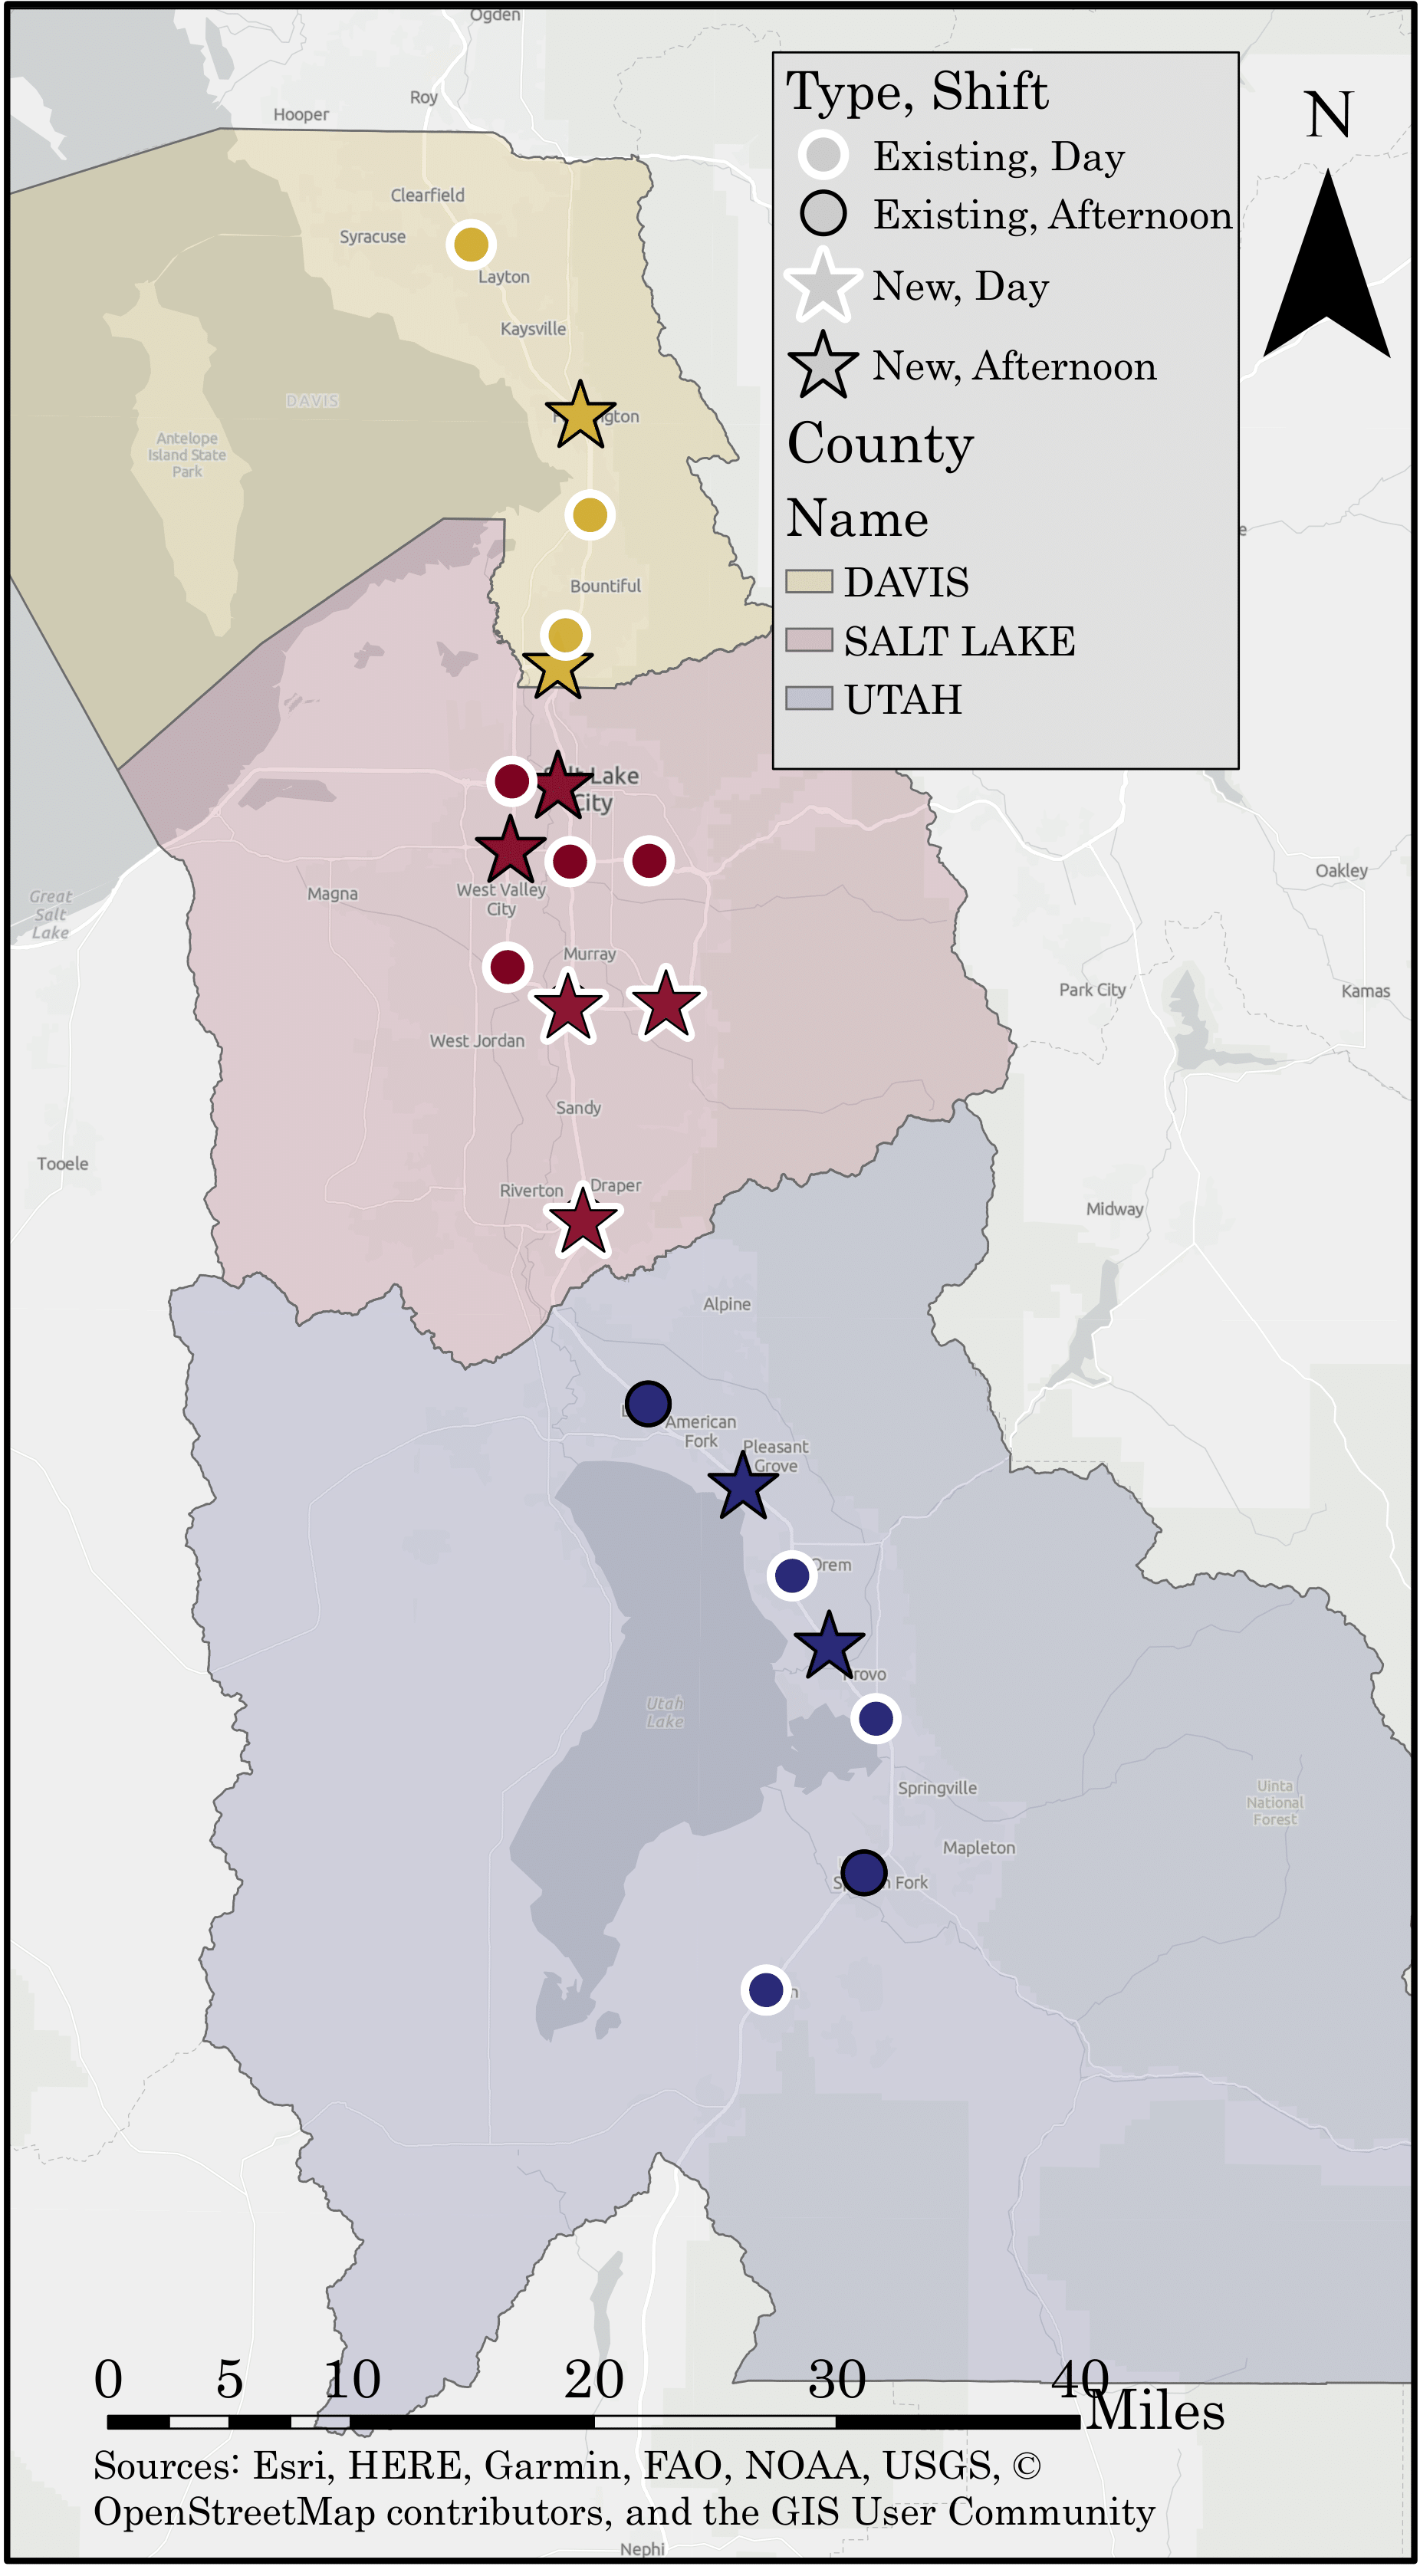
\includegraphics{figures/imt_gray_map.png}

}

\caption{\label{fig-IMT-Map}IMT starting locations example map.}

\end{figure}

Figure~\ref{fig-IMT-Map} uses circles to mark the locations of existing
IMT vehicles and stars for the proposed additions. We positioned these
units strategically along major highways to achieve a balanced
distribution of IMTs across each county. While this initial setup
doesn't mirror the real-world scenario where drivers begin their shifts
from home, it serves as a practical model for our simulations. The
frequency of IMT operations on major highways like I-15, I-80, and
I-215, along with the variable real-world starting points, justifies
this strategic alignment along key routes. Typically, IMT vehicles do
not cross county borders as dispatch services are organized by county.
However, in our MATSim network, vehicles can cross into other counties
depending on incident proximity. IMTs follow specific operational
shifts, which we've programmed into MATSim to reflect their
availability. In Utah, these often include a morning shift starting at
6:00 AM and an evening shift ending at 10:30 PM.
Figure~\ref{fig-IMT-Map} also illustrates the IMT distribution during
the evening shift, but it's important to note that this pattern is
generally consistent during the morning shift as well.

Our research primarily concentrates on evaluating the potential impacts
of expanding the IMT fleet, rather than examining the effects of their
starting positions. We hypothesize that increasing the number of IMTs,
assuming uniform distribution, will enhance their overall effectiveness.

\hypertarget{sec-inc_data}{%
\subsection{Incident Data and Sampling}\label{sec-inc_data}}

In their concurrent IMT research, Schultz et al. (2023) developed a
comprehensive dataset of incidents requiring management intervention,
derived from data provided by UHP. Analyzing data from 2018 to 2022,
they identified 1,604 incidents over 184 days that required the
assistance of either IMTs or UPH. This dataset is useful in
understanding the frequency of daily incidents in the Wasatch Front that
necessitate incident management intervention.
Figure~\ref{fig-incident-sampling-plot} illustrates the number incidents
in a given day on the x-axis and the number of days with that incident
frequency on its y-axis.

Figure~\ref{fig-incident-sampling-plot} demonstrates the ``Original
Distribution'' of observed daily incident frequencies in a bar chart
format. To simulate this distribution in our model, we used a randomized
sampling method to generate 10 distinct daily incident frequencies based
on the original data, labeled as the ``Current Frequency'' group. These
frequencies are represented as bars layered on top of the Original
Distribution in Figure~\ref{fig-incident-sampling-plot}. Additionally,
to assess IMT performance in scenarios with increased incident numbers,
we created a ``Increased Frequency'' group. This group includes the 10
highest daily incident frequencies from the original data and is
similarly layered over the ``Original Distribution'' in the
Figure~\ref{fig-incident-sampling-plot} bar chart.

\begin{figure}

{\centering \includegraphics{03_methods_files/figure-pdf/fig-incident-sampling-plot-1.pdf}

}

\caption{\label{fig-incident-sampling-plot}Sampling distributions for
incident frequencies.}

\end{figure}

From their established dataset of 1604 incidents Schultz et al. (2023)
filtered the data to ensure the completeness of each incident record in
the dataset, ensuring that the incident was responded to by an IMT and
contained complete information on incident duration, capacity reduction
and location, all of which are necessary for a comprehensive evaluation.
Filtering with those requirements they reduced the list to 411 unique
incidents that received IMT assistance.

Schultz et al. (2023) undertook concurrent IMT research and compiled a
comprehensive dataset of incidents requiring IMT intervention, drawing
on data from the UHP. They carefully ensured the completeness of each
incident record in the dataset, capturing crucial details such as the
incident start and end times, RCT, location, and extent of capacity
reduction.

Analyzing data from 2018 and 2022, Schultz et al. (2023) successfully
identified 1604 incidents over 184 days that required either IMT or UPH
assistance. The dataset they compiled provides insights into the
frequency of daily incidents in the Wasatch Front that are responded to
by incident management resources and is displayed in
Figure~\ref{fig-incident-sampling-plot} with the label ``Original
Distribution''. To represent that distribution of daily incidents in our
model, we used a randomized sampling technique to generate 10 distinct
values representing daily incident frequencies base on the ``Original
Distribution'' of the number of incidents in a given day. Those 10
values will be refereed to as the ``Current Incident Frequency'' or
``Current Frequency'' group and overlay the Original Distribution values
in Figure~\ref{fig-incident-sampling-plot}. Additionally, with the
desire to see how IMTs would preform with an elevated number of
incidents we formed a second sampling group called the ``Increased
Incident Frequency'' group, that was comprised of the 10 largest daily
incident frequencies from the original incident distribution.

From the list of 1604 incident they identified 411 unique incidents that
received IMT assistance and contained essential information on duration,
capacity reduction and location, all of which are necessary for a
comprehensive evaluation. We used this carefully curated dataset to
selectively include specific incidents in the MATSim model.

From that list of incidents they identified 411 unique incidents with
varying degrees of severity, ranging from property damage to fatal
incidents. We used this carefully curated dataset to selectively include
specific incidents in the MATSim model. It is important to acknowledge
that these 411 incidents only constitute a portion of all incidents
reported by UHP during this time frame. A number of additional incidents
were excluded from the analysis because they lacked essential
information on duration, capacity reduction, or location, all of which
are necessary for a comprehensive evaluation. Nevertheless, the
integration of the 411 analyzed incidents with the additional incomplete
records provides insights, aiding in quantifying the total number of
incidents within a specific time period. These combined incident records
informed the modeling of daily incident frequencies but were not used
for incident sampling in the simulation

To generate 10 distinct values representing daily incident frequencies,
we employed a randomized sampling technique. These values were
collectively termed Current Incident Frequencies as they were derived
from the original distribution of daily incidents. Furthermore, we
formulated a second set of 10 additional daily incident values, named
Increased Incident Frequencies. These values were extracted from the
upper portion of the 2022 incident data and were specifically designed
to assess the resilience and efficacy of the IMT system under scenarios
of markedly increased daily incidents. The visual depiction of the
original distribution of daily incidents, alongside the distributions
for both the Current and Increased Incident Frequencies, is illustrated
in Figure~\ref{fig-incident-sampling-plot}.

In total, 20 values were selected, evenly split with 10 allocated to the
Current Incident Frequency category, and the remaining 10 to the
Increased Incident Frequency category. Each value was subsequently
paired with a unique three-digit seed number, used internally within
MATSim to ensure a randomized selection of incidents for each simulation
scenario. Following this, we employed MATSim
\protect\hyperlink{sec-NCE}{network change events} to integrate the
incidents into the simulation.

\hypertarget{sec-scenarios}{%
\subsection{Scenarios}\label{sec-scenarios}}

In the \protect\hyperlink{sec-inc_data}{incident sampling} section and
Figure~\ref{fig-incident-sampling-plot}, we observe the establishment
and categorization of 20 distinct incident seeds into either Current or
Increased Incident frequencies. Each seed gave rise to three separate
simulation groups. The first group, No IMTs, exclusively features
simulations where incidents occur without any IMT intervention. The
second group includes incidents and the deployment of 20 IMTs, while the
third group features incidents managed by 30 IMTs.

In total, six scenario groups, each containing 10 random ``days'' with
distinct incident sets, were established, as follows:

\begin{itemize}
\tightlist
\item
  No IMTs, current incident frequency
\item
  No IMTs, increased incident frequency
\item
  20 IMTs, current incident frequency
\item
  20 IMTs, increased incident frequency
\item
  30 IMTs, current incident frequency
\item
  30 IMTs, increased incident frequency
\end{itemize}

It is important to note, as described in the
\protect\hyperlink{sec-IMT_setup}{IMT setup} section, that not all IMT
vehicles are operational simultaneously. Due to scheduling constraints,
the actual number of IMTs on the road at any given time is typically
half of the total fleet size.

Scenarios are evaluated by comparing each group with a baseline scenario
that assumes no incidents or IMT interventions. In this study, the
primary metrics for analyzing the traffic impact of incidents and IMTs
are the vehicle hours of delay (VHD) and RT. The MATSim outputs for each
scenario include the average delay per link over 15-minute periods.
Additionally, we compiled a file for each scenario documenting the
traffic volumes for each link during these time intervals. Multiplying
the traffic volumes by the average delays yields a detailed delay file,
which represents the aggregate delay on each network link for the
simulated ``day.'' The formula for calculating the link-specific delay
in a scenario is provided in Equation~\ref{eq-vhd_group}.

\begin{equation}\protect\hypertarget{eq-vhd_group}{}{
\text{VHD per link} = {\sum_{i=1}^{n} a_i}*{v_i}
}\label{eq-vhd_group}\end{equation} In Equation~\ref{eq-vhd_group},
\(a_i\) denotes the average delay for a link in the \(i^{th}\) time bin,
while \(v_i\) corresponds to the volume of vehicles traversing that link
during the same interval. The VHD for all links is summed to calculate
the total VHD for the entire network, and this total is further
categorized by motorway links and links directly affected by incidents.
For comparative analysis, the average VHD is computed across all
scenarios within each group. The analysis divides the average VHD into
three distinct categories: Network Links, Motorway Links, and Impacted
Links. Network Links provide a macroscopic view of network-wide delays,
Motorway Links focus on key routes such as highways and freeways, and
Impacted Links offer a detailed analysis of the delays at incident sites
and their immediate surroundings. This multi-tiered approach to analysis
facilitates a comprehensive evaluation of the widespread and specific
traffic impacts of incidents.

In addition to VHD, the study investigates the performance and
operational efficiency of IMTs. Metrics such as the average travel
times, travel distances, and incident RT are compared across the 20 IMT
and 30 IMT groups. This, in turn, informs strategic decisions regarding
resource allocation and deployment, ensuring that IMT vehicles are
optimally used to mitigate traffic delays and enhance roadway safety.

\bookmarksetup{startatroot}

\hypertarget{sec-results}{%
\chapter{Results}\label{sec-results}}

This section details the outcomes of the Utah IMT Optimization project,
employing the MATSim model to execute a series of simulations across a
range of scenario groups. Specifically, the groups---No IMTs, 20 IMTs,
and 30 IMTs---were compared with a Baseline scenario, facilitating an
evaluation of the repercussions of traffic incidents and the
effectiveness of IMTs in alleviating traffic disruptions.

The following sections analyze the results derived from the simulated
scenarios. This analysis uses VHD as a comparative metric examining
delay at the network, motorway, and incident links levels in sections
\protect\hyperlink{sec-VHD-Network}{4.1.1},
\protect\hyperlink{sec-VHD-Motorway}{4.1.2}, and
\protect\hyperlink{sec-impacted}{4.1.3}. The results also compare IMT
performance based on the teams average response times, total travel
time, and total travel distance in
\protect\hyperlink{sec-IMT-performance}{section 4.2}.

This analysis uses comparative metrics such as VHD, the consequences of
traffic incidents, and the dynamics of the IMT responses in relation to
the incidents they manage.

\hypertarget{vehicle-hours-of-delay}{%
\section{Vehicle Hours of Delay}\label{vehicle-hours-of-delay}}

The studies referenced in the \protect\hyperlink{sec-lit_imt_opt}{IMT
optimization} section of the
\protect\hyperlink{sec-literature}{literature review} demonstrate the
efficacy of IMTs in reducing RT and EUC on roadway segments affected by
incidents. Similarly, the results from this transportation model
highlight the impact of IMTs at reducing delay, particularly when
focusing on the segments of roadways where incidents occurred; see
section \protect\hyperlink{sec-impacted}{4.1.3}. In contrast to the
cited studies, our model also explored the broader implications of
incidents and their corresponding IMT responses on the simulated
network. In a majority of scenarios, these results also suggested a
strong positive correlation between IMTs and the reduction of RT and
VHD, which are key determinants in the computation of EUC.

\hypertarget{sec-VHD-Network}{%
\subsection{Network Hours of Delay}\label{sec-VHD-Network}}

In the comparison of network VHD across simulations, the scenarios were
grouped by IMT response and incident frequency. Each group encompassed
10 simulated scenarios, which each involved different selections and
number of incidents, with the exception of the Baseline scenario, which
stands alone. Table~\ref{tbl-network-delays-table} presents the average
VHD for each group, based on the delays recorded in the final iteration
of each simulation. These average VHD values are subsequently compared
against the Baseline scenario to calculate the percentage change in VHD.

\hypertarget{tbl-network-delays-table}{}
\begin{table}
\caption{\label{tbl-network-delays-table}Average VHD on Network }\tabularnewline

\centering
\begin{tabular}[t]{llrr}
\toprule
\textbf{Group} & \textbf{Incident Frequency} & \textbf{Average VHD} & \textbf{Change (\%)}\\
\midrule
\cellcolor{gray!6}{Baseline} & \cellcolor{gray!6}{-} & \cellcolor{gray!6}{74568} & \cellcolor{gray!6}{0.0}\\
No IMTs & Current & 103159 & 38.3\\
\cellcolor{gray!6}{No IMTs} & \cellcolor{gray!6}{Increased} & \cellcolor{gray!6}{104178} & \cellcolor{gray!6}{39.7}\\
20 IMTs & Current & 96697 & 29.7\\
\cellcolor{gray!6}{20 IMTs} & \cellcolor{gray!6}{Increased} & \cellcolor{gray!6}{95678} & \cellcolor{gray!6}{28.3}\\
\addlinespace
30 IMTs & Current & 93769 & 25.7\\
\cellcolor{gray!6}{30 IMTs} & \cellcolor{gray!6}{Increased} & \cellcolor{gray!6}{93560} & \cellcolor{gray!6}{25.5}\\
\bottomrule
\end{tabular}
\end{table}

Upon comparing the results across different groups, it was observed that
scenarios with 30 IMTs experienced the lowest average VHD. They were
closely followed by the 20 IMT group, and, as expected, the scenarios
that involved incidents only registered the highest average VHD values.
It is also noted that introducing incidents to the Baseline scenario
resulted in an average VHD increase of 39.0\%. However, this increase
dropped to an average of 29.0\% when 20 IMTs were available, and further
reduced to 25.6\% with the availability of 30 IMTs.

Additional analysis of the data revealed that, compared to the No IMTs
group, the 20 IMTs group decreased the average VHD by 7.2\%, while the
30 IMTs group reduced the average delay by 9.6\%. Lastly, when the 30
IMT and 20 IMT groups were compared against each other, the former
exhibited an average of 2.6\% less VHD than the latter.

While the relationship between the IMT group and VHD appeared
straightforward, the correlation between Incident Frequency and VHD was
not as clear-cut. In the No IMTs group, scenarios with increased
incident frequency showed only a 1.0\% increase in VHD compared to those
with the current frequency. Intriguingly, for both the 20 IMT and 30 IMT
groups, an increase in incident frequency actually led to slight
decreases in average VHD. The cause of this decrease is unclear, but
potential explanations will be discussed in the
\protect\hyperlink{sec-limitations}{limitations} section.

Given that Table~\ref{tbl-network-delays-table} reveals average delay
values aggregated across multiple scenarios within each group, a
graphical representation can enhance clarity regarding the inherent
variance within these data clusters.
Figure~\ref{fig-network-violin-plot} illustrates this data through
distribution plots.

\begin{figure}

{\centering \includegraphics{04_results_files/figure-pdf/fig-network-violin-plot-1.pdf}

}

\caption{\label{fig-network-violin-plot}Average network VHD
distribution.}

\end{figure}

In Figure~\ref{fig-network-violin-plot}, each distribution plot
represents the density distribution of delay values, with wider sections
indicating areas where numerous simulations converged around specific
delay values. Conversely, narrower sections suggest fewer simulations
clustering around those particular delay values. A dashed horizontal
line is superimposed to facilitate comparison of each group with the
results from the Baseline scenario. Additionally, diamond markers within
each plot denote the mean delay across all simulations in the respective
scenario group.

Upon examining these plots, we can make several observations. In the No
IMT group, the delay distribution for current incident frequencies is
broad, ranging from approximately 80,000 to 120,000 hours. However, with
an increase in incidents, VHD is more narrowly concentrated just above
100,000 hours. The distributions for the 20 IMT and 30 IMT plots each
show significant variance. Although the 30 IMT group tends to have lower
VHD than the 20 IMT group, a clear correlation between increased
incidents and network delay is not as evident as one might expect.
However, for the 20 IMT group with increased incidents, the widest
distribution segment is situated around 100,000 hours. In contrast, the
30 IMT group with increased incidents exhibits a broader distribution
near 90,000 hours, potentially indicating improved performance when
additional IMTs are made available.

While the preceding section discussed delays across the entire network,
it is important to note that all simulated incidents were located on
motorway links, predominantly along the major interstates of Utah's
Wasatch Front. This encompasses key routes such as I-15, I-80, and
I-215, as well as other significant freeways and highways. The
subsequent section will provide a detailed analysis of the simulation
outcomes specifically related to these motorway links.

\hypertarget{sec-VHD-Motorway}{%
\subsection{Motorway Link Hours of Delay}\label{sec-VHD-Motorway}}

The network used in our model is derived from the Wasatch Front Regional
Council travel demand model network. Within this network, the term
`motorway' denotes a specific type of link, also known as a freeway or
expressway in different contexts. To ensure consistency throughout this
document, we primarily refer to these road segments as `motorway' or
`motorway links.' It is important to note, however, that in the
simulation, incidents can occur on both interstates and major highways
along the Wasatch Front.

To compare average simulation performances,
Table~\ref{tbl-motorway-delays-table} breaks down the average motorway
VHD for each group, categorized by IMT response and incident frequency.
Table~\ref{tbl-motorway-delays-table} reveals that, in comparison to the
Baseline scenario, the average VHD on motorway links increased by
approximately 7,000-9,000 hours, or 45.6-58.1\%, when incidents were
introduced. The 20 IMT group, on average, exhibited a 24.2\% increase in
VHD from the Baseline, whereas the 30 IMT group experienced an average
VHD increase of 17.0\%.

\hypertarget{tbl-motorway-delays-table}{}
\begin{table}
\caption{\label{tbl-motorway-delays-table}Average VHD of Motorway Links }\tabularnewline

\centering
\begin{tabular}[t]{llrr}
\toprule
\textbf{Group} & \textbf{Incident Frequency} & \textbf{Average VHD} & \textbf{Change (\%)}\\
\midrule
\cellcolor{gray!6}{Baseline} & \cellcolor{gray!6}{-} & \cellcolor{gray!6}{15335} & \cellcolor{gray!6}{0.0}\\
No IMT & Current & 24242 & 58.1\\
\cellcolor{gray!6}{No IMT} & \cellcolor{gray!6}{Increased} & \cellcolor{gray!6}{22321} & \cellcolor{gray!6}{45.6}\\
20 IMT & Current & 18924 & 23.4\\
\cellcolor{gray!6}{20 IMT} & \cellcolor{gray!6}{Increased} & \cellcolor{gray!6}{19176} & \cellcolor{gray!6}{25.0}\\
\addlinespace
30 IMT & Current & 17569 & 14.6\\
\cellcolor{gray!6}{30 IMT} & \cellcolor{gray!6}{Increased} & \cellcolor{gray!6}{18327} & \cellcolor{gray!6}{19.5}\\
\bottomrule
\end{tabular}
\end{table}

At the motorway link level, the differences between the No IMT group and
the IMT groups becomes more pronounced than they were for delays across
the entire network. Specifically, the 20 IMT group demonstrated an
average 18.2\% decrease in VHD compared to the No IMT group, while the
30 IMT group showed an average 22.9\% decrease in VHD.

Interestingly, the difficulty in correlating VHD with incident frequency
observed in Table~\ref{tbl-network-delays-table} manifests differently
in Table~\ref{tbl-motorway-delays-table}. The latter indicates that,
within the IMT groups, an increase in incident frequency corresponds
with an increase in VHD. Specifically, the 20 IMT group experiences an
average VHD increase of 1.3\% when transitioning from current to
increased incident frequencies, while the 30 IMT group sees a 4.3\%
uptick under the same conditions. In contrast, and quite unexpectedly,
the No IMT group shows a 7.9\% reduction in VHD when comparing scenarios
of current and increased incident frequencies. This finding is
particularly perplexing given that Table~\ref{tbl-network-delays-table}
suggests an overall increase in VHD across the entire network for the No
IMT group when incident frequency increases.

A potential explanation for these unexpected VHD outcomes on motorway
links could be that, as part of their scoring and replanning process,
some MATSim agents opted for travel on non-motorway links to reach their
destinations. This would essentially redistribute the delay from
motorway links to other parts of the network.

For a better understanding of the variances within the scenario groups,
Figure~\ref{fig-motorway-violin-plot} may provide additional insights.
In Figure~\ref{fig-motorway-violin-plot}, we observe distinct patterns
in the distribution of delays for different scenario groupings. Key
observations include:

\begin{figure}

{\centering \includegraphics{04_results_files/figure-pdf/fig-motorway-violin-plot-1.pdf}

}

\caption{\label{fig-motorway-violin-plot}Average motorway VHD
distribution.}

\end{figure}

\begin{itemize}
\tightlist
\item
  A wide span across the plots for both groupings of No IMT, indicating
  a significant variance in delays across those simulations.
\item
  A concentration of delays around the Baseline value of 15,000 VHD for
  both the 20 IMT and 30 IMT scenarios, as shown by the width of the
  plots at this point.
\item
  A narrowing of the IMT group plots as they transition to higher delay
  values, suggesting fewer instances of extreme delays.
\item
  The upper tails of the 20 IMT plots extend beyond those of the 30 IMT
  plots, suggesting that the 30 IMT fleet may be more effective at
  mitigating delays in outlier scenarios compared to the 20 IMT fleet.
\end{itemize}

\hypertarget{sec-impacted}{%
\subsection{Impacted Links}\label{sec-impacted}}

The final section of our VHD analysis delves into the delays experienced
on incident links and their immediate upstream counterparts. This level
of analysis aligns with the methodologies employed in the studies by
Bennett et al. (2021) and Skabardonis (1998), as it focuses on the most
direct repercussions of incidents and IMTs. Unlike their focus on the
impacts of IMTs on RCT, our investigation centers on VHD as an indicator
of EUC. As detailed in the \protect\hyperlink{sec-imt_response}{IMT
assignment and response} section, the IMTs in our simulation did not
curtail the duration of incidents (RCT); instead, they enhanced roadway
capacity. Nonetheless, given that EUC is intrinsically related to delay,
this section offers an evaluation of IMT performance similar to the
analyses conducted by Bennett et al. (2021) and Skabardonis (1998).

Impacted links examines VHD on incident links and their immediate
upstream counterparts. Given the variation in link lengths across the
motorway, in some cases, analyzing just two additional links may not
fully capture the delays caused by a specific incident. Nevertheless,
Table~\ref{tbl-impacted-links} provides insights into how delays on
impacted links vary based on incidents and IMT deployment. For
additional context about Table~\ref{tbl-impacted-links}: `Total VHD'
represents the delay on impacted links both during the incidents and for
one hour after clearance, aiming to capture any residual delay shock
waves that an incident might cause.

\hypertarget{tbl-impacted-links}{}
\begin{table}
\caption{\label{tbl-impacted-links}Impacted Links Delay }\tabularnewline

\centering
\begin{tabular}[t]{llrr}
\toprule
\textbf{Group} & \textbf{Incident Frequency} & \textbf{Total VHD} & \textbf{Avg. Delay Per Inc. [hrs.]}\\
\midrule
\cellcolor{gray!6}{Baseline} & \cellcolor{gray!6}{Current} & \cellcolor{gray!6}{326} & \cellcolor{gray!6}{3.6}\\
No IMT & Current & 3808 & 42.3\\
\cellcolor{gray!6}{20 IMT} & \cellcolor{gray!6}{Current} & \cellcolor{gray!6}{723} & \cellcolor{gray!6}{8.0}\\
30 IMT & Current & 366 & 4.1\\
\cellcolor{gray!6}{Baseline} & \cellcolor{gray!6}{Increased} & \cellcolor{gray!6}{540} & \cellcolor{gray!6}{2.8}\\
\addlinespace
No IMT & Increased & 3154 & 16.3\\
\cellcolor{gray!6}{20 IMT} & \cellcolor{gray!6}{Increased} & \cellcolor{gray!6}{1645} & \cellcolor{gray!6}{8.5}\\
30 IMT & Increased & 1115 & 5.8\\
\bottomrule
\multicolumn{4}{l}{\textsuperscript{a} Note: Current contains 90 incidents, Increased contains 193}\\
\end{tabular}
\end{table}

Table~\ref{tbl-impacted-links} presents a division of the Baseline
scenario into two segments, for a more accurate comparison with the
other three scenarios. Despite the absence of incidents in the Baseline
scenario, its delay values are derived from the same links included in
the other scenario calculations.

The data in Table~\ref{tbl-impacted-links} indicate that the 30 IMT
group delay patterns align most closely with the Baseline. They are
followed by the 20 IMT group, and subsequently, the No IMT group. It is
important to note that directly comparing the Total VHD of the Current
and Increased incident groups may not be appropriate due to variations
in sample sizes, as noted in Table~\ref{tbl-impacted-links}. A more apt
comparison might be to evaluate the average delay experienced per
incident. Using this parameter, we observe an increase in the average
VHD for both the 20 and 30 IMT groups, correlating with an uptick in the
number of incidents. However, the scenarios involving No IMTs yield a
different outcome: both Total VHD and the average delay per incident
exhibit a decrease when the incident frequency increased. A more close
examination of the data draws attention to a particular scenario, Seed
141, which contributed an exceptionally large delay to the incident
links in the Current Incident category. This anomaly could potentially
explain the seemingly unexpected findings observed in the No IMTs,
Current Incident frequency scenarios.

For a more detailed analysis, the scatter plot in
Figure~\ref{fig-impacted-links-plot} categorizes the data based on seed
type. On the y-axis, the labels represent a combination of incident
numbers and seed values, with the format ``number\_seed'' (e.g.,
``12\_141'' denotes a scenario involving 12 incidents associated with
seed value 141).

\begin{figure}

{\centering \includegraphics{04_results_files/figure-pdf/fig-impacted-links-plot-1.pdf}

}

\caption{\label{fig-impacted-links-plot}Delay on impacted links.}

\end{figure}

Figure~\ref{fig-impacted-links-plot} offers a detailed view of the VHD
on impacted links across the simulated scenarios. At a glance, the
Baseline and 30 IMT scenarios, represented by blue and orange dots, seem
to predominantly cluster to the left of the pink dots, which depict the
No IMT scenarios. However, a more thorough analysis reveals that in
specific instances, the 20 IMT, 30 IMT, or even both scenarios may
underperform compared to the No IMT scenarios. This seemingly unexpected
observation suggests that there may be additional factors, aside from
link capacity, affecting the delay.

It is important to acknowledge the inherent dynamic nature of the MATSim
iterative process, where the ways in which agents re-plan their journeys
can sometimes have as significant, or potentially even greater, impact
on delays than changes in link capacity due to incidents or IMTs.
Importantly, in scenarios with the highest delays, the introduction of
IMTs seems to considerably reduce delay on the affected links.

Note that the x-axis has been limited to a maximum of 400+ VHD. This
limit enhances the visibility of the majority of data points. Without
this adjustment, the outlier point from the No IMT scenario with seed
141, which reported over 1,000 hours of delay, would have necessitated a
much wider scale, potentially obscuring the trends and patterns in the
rest of the data.

\hypertarget{sec-IMT-performance}{%
\section{IMT Performance Analysis}\label{sec-IMT-performance}}

Equally critical to understanding IMT performance is assessing the
efficiency of each IMT in reaching their intended destinations. This
results segment delves into IMT travel behavior, capturing metrics such
as average travel times and distances, along with their average incident
response times. The analysis encompasses both 20 IMT and 30 IMT
scenarios.

Travel times for IMTs can be extracted from the event files, which are
produced as a standard MATSim output. These files provide insights into
the distance and time traveled by each IMT. Utilizing this IMT travel
data, plots were generated to illustrate the average travel times and
distances for each dispatched IMT within a given scenario.
Figure~\ref{fig-truck-time-plot} illustrates the average travel time for
each dispatched IMT.

\begin{figure}

{\centering \includegraphics{04_results_files/figure-pdf/fig-truck-time-plot-1.pdf}

}

\caption{\label{fig-truck-time-plot}Average daily IMT travel time per
dispatched team.}

\end{figure}

To compute the average travel time per IMT we took the cumulative travel
time for all dispatched IMTs in every scenario and divided that by the
number of teams deployed. Furthermore, an analysis of the IMT travel
data reveals that scenarios with 30 IMT generally dispatched more units
than scenarios with only 20 IMT. A nearly analogous methodology was
employed to generate Figure~\ref{fig-truck-distance-plot}.

Similar to the observed differences in IMT travel times across various
scenarios, a distinct difference is apparent in the average distance
traversed per dispatched IMT between the 20 IMT and 30 IMT scenarios.
This pattern is illustrated in Figure~\ref{fig-truck-distance-plot},
clearly demonstrating a correlation between a higher quantity of IMTs
and a reduced average distance traveled per team.

\begin{figure}

{\centering \includegraphics{04_results_files/figure-pdf/fig-truck-distance-plot-1.pdf}

}

\caption{\label{fig-truck-distance-plot}Average daily IMT travel
distance per dispatched team.}

\end{figure}

Altering the starting locations of the IMTs or having them operate in a
roaming manner, as opposed to starting from a stationary location, can
significantly influence the time and distance traveled, presenting both
potential advantages and drawbacks (Lou et al., 2011). Although various
factors, including fleet size and vehicle starting locations, were
highlighted by Lou et al. (2011) as impactful in influencing IMT
response times, it is important to clarify that determining the optimal
starting points for IMTs was not the primary focus of UDOT in this
research. This aspect, while not explored in the current study, presents
a valuable opportunity for future research, opening up an intriguing
avenue for investigations using the ImtModule MATSim extension
associated with this report.

In the study conducted by Bennett et al. (2021), it is highlighted that
in Utah, a one-minute increase in IMT response time results in an
approximate 0.8-minute increase in RCT. This finding emphasizes the
critical role of IMTs response times in reducing RCT and subsequent
delays. While not examining RCT, this study also investigated the RT of
IMT when dispatching both 20 and 30 units. As indicated in
Table~\ref{tbl-truck-arrival-table}, across all simulated scenarios, a
fleet of 20 IMTs produced an average incident RT of 15.0 minutes.
Notably, the 15.0-minute average arrival time for the 20 IMT scenarios
aligns closely with the actual median arrival times recorded in Hyer's
2023 study of Utah's IMT performance (Schultz et al., 2023).
Additionally, increasing the IMT fleet to 30 units resulted in an
average response time of 11.0 minutes, 4 minutes less than the 20 IMT
group arrival times. Table~\ref{tbl-truck-arrival-table} illustrates the
average arrival times of the 1st, 2nd, and 3rd IMT, as well as the
average for all units' arrival times.

\hypertarget{tbl-truck-arrival-table}{}
\begin{table}
\caption{\label{tbl-truck-arrival-table}Average IMT Arrival Times }\tabularnewline

\centering
\begin{tabular}[t]{lllll}
\toprule
\textbf{Group} & \textbf{All IMT [mins]} & \textbf{1st [mins]} & \textbf{2nd [mins]} & \textbf{3rd [mins]}\\
\midrule
\cellcolor{gray!6}{20 IMTs} & \cellcolor{gray!6}{15.0} & \cellcolor{gray!6}{11.1} & \cellcolor{gray!6}{21.1} & \cellcolor{gray!6}{28.9}\\
30 IMTs & 11.0 & 8.9 & 13.2 & 21.2\\
\cellcolor{gray65}{\cellcolor{gray!6}{Number of Incidents}} & \cellcolor{gray65}{\cellcolor{gray!6}{280}} & \cellcolor{gray65}{\cellcolor{gray!6}{280}} & \cellcolor{gray65}{\cellcolor{gray!6}{116}} & \cellcolor{gray65}{\cellcolor{gray!6}{23}}\\
\bottomrule
\end{tabular}
\end{table}

Table~\ref{tbl-truck-arrival-table} provides insights into the IMT
response patterns, capturing their arrival at 280 out of 283 incidents
across both scenarios. Note, three unattended incidents fell outside of
the IMT operational hours. Among the incidents that were managed,
support from a second IMT was requested 116 times, from a third IMT 23
times, and a fourth IMT was called upon 3 times. However, due to the
extremely small number of incidents requiring a fourth IMT, this
category was deemed too limited for significant analysis and was
subsequently excluded from Table~\ref{tbl-truck-arrival-table}. When
comparing arrival times, scenarios with 30 IMTs consistently
outperformed those with 20 IMTs, demonstrating quicker response times
across all incident categories. As noted earlier, the average RT with 30
IMTs was 4 minutes shorter than with 20 IMTs. Hadfield et al. (2021)
estimated that a one-minute delay in RT added 34.6 minutes to the
estimated travel time, and an increase of \$925 in EUC. Based on these
findings, reducing the RT of IMTs by an average of 4 minutes could
result in EUC savings of approximately \$3,700 per incident.

A closer analysis of the IMT travel data reveals significant insights
into operational efficiency. The data indicate that the group with 30
IMTs was markedly more efficient than the group with 20 IMTs.
Specifically, the 20 IMT group accumulated a total of 105 hours of
travel time, while the 30 IMT group managed to reduce this to 77
hours---a significant decrease of 27\% in total IMT travel time.
Additionally, the data show that with 20 IMTs, units were often
dispatched to multiple incidents in quick succession, negatively
impacting their arrival times. In contrast, the scenarios with 30 IMTs,
supported by a larger fleet, saw fewer instances of consecutive
deployments, leading to more timely arrivals. This increased efficiency
with the 30 IMT group becomes particularly evident in high-frequency
incident situations, especially when comparing the arrival times of the
2nd and 3rd IMT between the two scenario groups.

\hypertarget{results-summary}{%
\section{Results Summary}\label{results-summary}}

We evaluated the impact of deploying fleets of 20 and 30 IMTs using our
MATSim model, enhanced with an IMT analysis extension, comparing these
scenarios to ones without IMT support. Our findings suggest that IMTs
are effective in reducing VHD on roadways and in decreasing incident
response times. However, a number of simulation results yielded some
unexpected outcomes. We will delve into these discrepancies in the
\protect\hyperlink{sec-limitations}{limitations section} of our
conclusions. A notable shortcoming of our MATSim model was its absence
of a `within-day replanning' feature, which is useful for accurately
simulating real-world responses to unforeseen events. This omission
might account for some of the variances observed in our results.
Therefore, while our findings offer valuable insights, the model
requires further refinement and calibration before it can reliably
inform policy or operational strategies. Nonetheless, with minor
enhancements to our modeling approach, the MATSim model demonstrates
potential as an effective tool for future analysis of IMT performance
and operations at UDOT.

\bookmarksetup{startatroot}

\hypertarget{sec-conclusions}{%
\chapter{Conclusions}\label{sec-conclusions}}

This paper contributes to the existing body of knowledge on IMT
effectiveness and traffic incident modeling. It highlights the
importance of strategic IMT deployment and the necessity for ongoing
evaluation and adaptation of these strategies to meet changing demands
in highway operational systems. Our study focuses on the Utah Wasatch
Front Region, employing simulation modeling to evaluate IMT
effectiveness. Previous studies have established IMT's significance in
mitigating traffic disruptions, such as incidents and vehicle breakdowns
(Bennett et al., 2022; Hadfield et al., 2021; Schultz et al., 2023;
Skabardonis, 1998). Furthermore, mesoscopic DTA modeling has proven
beneficial for in-depth analyses of incident impacts and management
strategies {[}Kaddoura \& Nagel (2018); Li \& Ferguson (2020);
sisiopiku2007{]}.

However, there is a noticeable lack of large-scale simulation models
applied to evaluating IMT performance. These models offer unique
insights and enable scenario testing that may be challenging with
traditional methods. To address this gap, we developed a specific
simulation model for assessing IMT operations across Utah, seeking to
improve our understanding and the effectiveness of these teams.

We used our model to analyze VHD and various IMT performance measures
across different incident types and IMT configurations. Our analysis
primarily focused on comparing the outcomes based on the number of IMT
deployed in each scenario. The results indicated that the existing fleet
of 20 IMTs deployed by UDOT effectively respond to incidents and reduce
delay. In comparison to scenarios with incidents alone, a 20 IMT
configuration reduced highway delays by 18.2\%, resulting in an average
VHD reduction of 4232 hours per simulated day. Increasing the fleet size
to 30 IMTs led to a reduction in delay of 22.9\% and an average VHD
savings of 5334 hours.

Additionally, in our simulation, a fleet of 30 IMTs showed quicker
response times to incidents compared to a fleet of 20 IMTs, with average
response times decreasing from 15.0 minutes to 11.0 minutes. Notably,
the 15.0-minute average arrival time for the 20 IMT scenarios aligns
closely with the actual median arrival time recorded in Hyer's 2023
study on Utah IMT performance (Schultz et al., 2023). Additionally,
increasing the IMT fleet to 30 resulted in a cumulative reduction of 28
hours in travel time across 20 scenarios. This translates to an average
decrease of 1.4 hours in IMT travel time per simulated day.

\hypertarget{sec-implications}{%
\section{Implications}\label{sec-implications}}

In their study on Utah's IMT performance, Hadfield et al. (2021) found
that a one-minute delay in IMT response time led to a 0.8-minute
increase in RCT, an additional 34.6 minutes in total estimated travel
time, and an increase of \$925 in EUC. Building on these findings, we
estimate that reducing the IMT response time by an average of 4 minutes
--- a potential outcome of adding 10 more IMTs to the fleet --- could
result in EUC savings of approximately \$3,700 per incident.

As UDOT evaluates the effectiveness of their IMT program and
contemplates potential expansion, this study's insights become a crucial
asset for informed decision-making. Our
\protect\hyperlink{sec-results}{results} suggest that increasing the IMT
fleet has the potential to decrease VHD and enhance the speed of
incident response.

The model we developed for this project addresses two significant
`what-if' scenarios, applicable to UDOT or any other transportation
agency aiming to optimize their IMT program:

\begin{enumerate}
\def\labelenumi{\arabic{enumi}.}
\tightlist
\item
  What if the incidence of traffic disruptions in our region surges? How
  might this impact our incident management program's effectiveness?
\item
  What if we decide to increase the size of our IMT fleet? What are the
  potential advantages and potential challenges associated with this
  expansion?
\end{enumerate}

While our primary objective was to address these scenarios, the model's
versatility enables future exploration of additional questions, such as:

\begin{itemize}
\tightlist
\item
  Identifying the optimal deployment locations for IMTs in our system.
\item
  Assessing whether the current operational hours of the IMT program are
  optimal.
\end{itemize}

\hypertarget{sec-limitations}{%
\section{Limitations}\label{sec-limitations}}

The limitations of this study are mainly attributed to the model we
developed and the aspects that can be enhanced. As outlined in the
\protect\hyperlink{sec-inc_modeling}{incident modeling} section, we
opted for MATSim to simulate IMT performance due to its ability to
handle large-scale networks, incorporate real-world data, and mimic
authentic driver behavior. While MATSim can realistically portray driver
behavior, employing additional methods could have further enhanced its
performance in our simulations.

In the \protect\hyperlink{sec-MATSim_Score}{scoring and replanning}
section, we describe how agents in MATSim alter their routes through an
iterative scoring process influenced by various factors including late
arrival, mode choice, and activity type. Although this method is
generally effective, it may present challenges when simulating
unforeseen events like traffic incidents.

As Dobler et al. (2012) highlight in their chapter of the MATSim manual,
employing a within-day replanning tool is helpful within the MATSim
framework, especially for handling unexpected situations. They note that
while the iterative modeling approach of MATSim is adept at reaching
user equilibrium under typical conditions, it tends to falter during
sudden events. This can result in seemingly irrational behaviors, such
as agents changing routes before an incident actually takes place.

The scenario depicted in Figure \ref{fig-within-day} serves as an
illustrative example of the potential routing issues that can arise in
MATSim when within-day replanning is not applied. In this instance, an
agent is navigating from a start point marked by the red dot to a
destination marked by the green dot. At 14:02, a traffic incident
disrupts the agent's original route. Nevertheless, due to the
anticipatory nature of MATSim's iterative approach, the agent already
reroutes at 14:00---2 minutes before the incident occurs. This early
route change showcases the challenges of solely relying on an iterative
modeling strategy for responding to sudden events. It also emphasizes
the benefit of incorporating a within-day replanning feature, which
relies on a single iteration to provide more accurate and realistic
navigational adjustments.

\begin{figure}
\centering
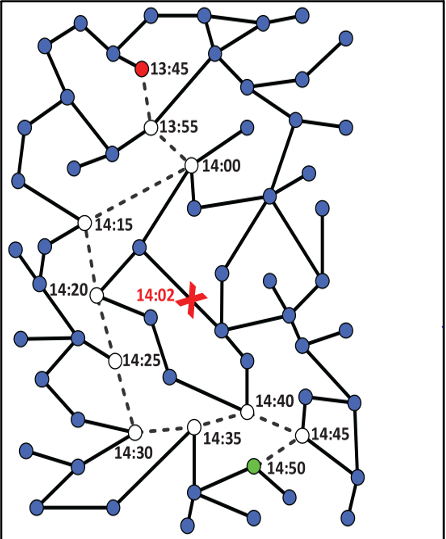
\includegraphics{figures/within_day.png}
\caption[Within-day replanning approach for a MATSim routing problem.]{Within-day replanning approach for a MATSim routing problem (Dobler et al., 2012).}
\label{fig-within-day}
\end{figure}

Unfortunately, the problem showcased in Figure \ref{fig-within-day}
surfaced at times throughout our MATSim simulations. In certain
scenarios, agents would have preemptively avoided specific road links
anticipated to have incidents, rather than adhering to more realistic
behavior patterns observed on real roads. Typically, drivers maintain
their intended course until directly confronted with congestion or
delays, at which point they may choose to reroute. This variance between
the simulated and actual driver responses to unforeseen road incidents
underscores a key area for enhancement in our simulation model, ensuring
it more accurately reflects realistic driving behavior.

\hypertarget{sec-next_steps}{%
\section{Next Steps}\label{sec-next_steps}}

Moving forward, enhancing the simulation of IMT response and performance
could be achieved by implementing the adjustments mentioned in the
\protect\hyperlink{sec-limitations}{limitations}, specifically
concerning the replanning and configuration settings of the MATSim
model. Future steps could also involve exploring additional methods for
simulated analysis of IMT performance measures. Depending on the
specific requirements of UDOT or other transportation agencies, the
simulation could be modified to evaluate optimal IMT starting locations,
hours of operation, or their overall cost-benefit ratio.

Overall, the simulation we developed largely corroborates previous
findings regarding the efficacy of IMTs. While it necessitates certain
adjustments to enhance its reliability, it demonstrates potential as a
tool for examining IMT performance in ways that previous studies have
not.

\bookmarksetup{startatroot}

\hypertarget{references}{%
\chapter*{References}\label{references}}
\addcontentsline{toc}{chapter}{References}

\markboth{References}{References}

\hypertarget{refs}{}
\begin{CSLReferences}{1}{0}
\leavevmode\vadjust pre{\hypertarget{ref-bennett2021}{}}%
Bennett, L. S., Hadfield, M. G., Schultz, G. G., Saito, M., \& Eggett,
D. L. (2021). Performance measures evaluation of UDOT's traffic incident
management program. \emph{Proceedings of the International Conference on
Transportation \& Development 2021: Transportation Operations,
Technologies, and Safety}, 25--36.

\leavevmode\vadjust pre{\hypertarget{ref-bennett2022}{}}%
Bennett, L. S., Schultz, G. G., Hyer, J., Saito, M., \& Eggett, D. L.
(2022). The benefits of expanding the incident management program in
utah. \emph{Proceedings of the International Conference on
Transportation \& Development 2022: Transportation Safety}, 264--276.

\leavevmode\vadjust pre{\hypertarget{ref-chiu2011}{}}%
Chiu, Y.-C., Bottom, J., Mahut, M., Paz, A., Balakrishna, R., Waller,
T., \& Hicks, J. (2011). Dynamic traffic assignment: A primer.
\emph{Transportation Research Circular}.
\url{https://api.semanticscholar.org/CorpusID:15677103}

\leavevmode\vadjust pre{\hypertarget{ref-day2023}{}}%
Day, C. S., Macfarlane, G. S., Erhardt, G. D., \& Watkins, K. (2023).
\emph{MMOS integration -- forecasting ride-hailing across multiple model
frameworks} (TSCORE-M3). Transit -- Serving Communities Optimally,
Responsively,; Efficiently (T-SCORE) Center {[}UTC{]}; Brigham Young
University; University of Kentucky; University of California, Davis.
\url{https://rosap.ntl.bts.gov/view/dot/67058}

\leavevmode\vadjust pre{\hypertarget{ref-dia2006}{}}%
Dia, H., \& Cottman, N. (2006). Evaluation of arterial incident
management impacts using traffic simulation. \emph{Intelligent Transport
Systems, IEE Proceedings}, \emph{153}, 242--252.
\url{https://doi.org/10.1049/ip-its:20055005}

\leavevmode\vadjust pre{\hypertarget{ref-dobler2012}{}}%
Dobler, C., Kowald, M., Rieser-Schüssler, N., \& Axhausen, K. W. (2012).
Within-day replanning of exceptional events. \emph{Transportation
Research Record}, \emph{2302}(1), 138--147.
\url{https://doi.org/10.3141/2302-15}

\leavevmode\vadjust pre{\hypertarget{ref-hadfield2021}{}}%
Hadfield, M. G., Bennett, L. S., Schultz, G. G., Saito, M., \& Eggett,
D. L. (2021). User cost analysis of UDOT's traffic incident management
program. \emph{Proceedings of the International Conference on
Transportation \& Development 2021: Transportation Planning and
Development}, 71--82.

\leavevmode\vadjust pre{\hypertarget{ref-horni2016}{}}%
Horni, A., \& Nagel, K. (2016). More about configuring MATSim. In A.
Horni, K. Nagel, \& K. W. Axhausen (Eds.), \emph{The multi-agent
transport simulation MATSim} (pp. 35--44). Ubiquity Press.
\url{https://doi.org/10.5334/baw.4}

\leavevmode\vadjust pre{\hypertarget{ref-kaddoura2018}{}}%
Kaddoura, I., \& Nagel, K. (2018). Using real-world traffic incident
data in transport modeling. \emph{Procedia Computer Science},
\emph{130}, 880--885. \url{https://doi.org/10.1016/j.procs.2018.04.084}

\leavevmode\vadjust pre{\hypertarget{ref-kim2012}{}}%
Kim, W., Franz, M., Chang, G.-L., \& University of Maryland (College
Park, Md. ). Dept. of C. and E. E. (2012). \emph{Enhancement of freeway
incident traffic management and resulting benefits.}

\leavevmode\vadjust pre{\hypertarget{ref-li2020}{}}%
Li, J., \& Ferguson, N. (2020). A multi-dimensional rescheduling model
in disrupted transport network using rule-based decision making.
\emph{Procedia Computer Science}, \emph{170}, 90--97.
\url{https://doi.org/10.1016/j.procs.2020.03.012}

\leavevmode\vadjust pre{\hypertarget{ref-lou2011}{}}%
Lou, Y., Yin, Y., \& Lawphongpanich, S. (2011). Freeway service patrol
deployment planning for incident management and congestion mitigation.
\emph{Transportation Research Part C: Emerging Technologies},
\emph{19}(2), 283--295. \url{https://doi.org/10.1016/j.trc.2010.05.014}

\leavevmode\vadjust pre{\hypertarget{ref-macfarlane2023}{}}%
Macfarlane, G., \& Lant, N. (2023). \emph{How far are we from
transportation equity? Measuring the effect of wheelchair use on daily
activity patterns} (pp. 141--155).
\url{https://doi.org/10.1007/978-981-19-8361-0_10}

\leavevmode\vadjust pre{\hypertarget{ref-nagel2016}{}}%
Nagel, K., Kickhöfer, B., Horni, A., \& Charypar, D. (2016). A closer
look at scoring. In A. Horni, K. Nagel, \& K. W. Axhausen (Eds.),
\emph{The multi-agent transport simulation MATSim} (pp. 23--34).
Ubiquity Press. \url{https://doi.org/10.5334/baw.3}

\leavevmode\vadjust pre{\hypertarget{ref-owens2010}{}}%
Owens, N., Armstrong, A., Sullivan, P. E., Mitchell, C., Newton, D.,
Brewster, R. M., \& Trego, T. G. (2010). \emph{Traffic incident
management handbook}.
\url{https://api.semanticscholar.org/CorpusID:106965152}

\leavevmode\vadjust pre{\hypertarget{ref-ozbay2013}{}}%
Ozbay, K., Iyigun, C., Baykal-Gursoy, M., \& Xiao, W. (2013).
Probabilistic programming models for traffic incident management
operations planning. \emph{Annals of Operations Research},
\emph{203}(1), 389--406. \url{https://doi.org/10.1007/s10479-012-1174-6}

\leavevmode\vadjust pre{\hypertarget{ref-pal2002}{}}%
Pal, R., \& Sinha, K. C. (2002). Simulation model for evaluating and
improving effectiveness of freeway service patrol programs.
\emph{Journal of Transportation Engineering}, \emph{128}(4), 355--365.
\url{https://doi.org/10.1061/(ASCE)0733-947X(2002)128:4(355)}

\leavevmode\vadjust pre{\hypertarget{ref-rieser2016}{}}%
Rieser, M., Nagel, K., \& Horni, A. (2016). MATSim data containers. In
A. Horni, K. Nagel, \& K. W. Axhausen (Eds.), \emph{The multi-agent
transport simulation MATSim} (pp. 55--60). Ubiquity Press.
\url{https://doi.org/10.5334/baw.6}

\leavevmode\vadjust pre{\hypertarget{ref-schultz2023}{}}%
Schultz, G. G., Hyer, J., Holdsworth, W. H., Eggett, D. L., \&
Macfarlane, G. S. (2023). \emph{Analysis of benefits of UDOT's expanded
incident management team program} (UT-23.05). Utah Department of
Transportation Research \& Innovation Division.

\leavevmode\vadjust pre{\hypertarget{ref-sisiopiku2007}{}}%
Sisiopiku, V. P., Li, X., Mouskos, K. C., Kamga, C., Barrett, C., \&
Abro, A. M. (2007). Dynamic traffic assignment modeling for incident
management. \emph{Transportation Research Record}, \emph{1994}(1),
110--116. \url{https://doi.org/10.3141/1994-15}

\leavevmode\vadjust pre{\hypertarget{ref-skabardonis1998}{}}%
Skabardonis, A. (1998). \emph{Evaluation of the freeway service patrol
(FSP) in los angeles} (PATH Research Report UCB-ITS-PRR-98-31).
University of California, Berkeley, California PATH Program, Institute
of Transportation Studies.
\url{https://escholarship.org/uc/item/3920p806}

\leavevmode\vadjust pre{\hypertarget{ref-wirtz2005}{}}%
Wirtz, J. J., Schofer, J. L., \& Schulz, D. F. (2005). Using simulation
to test traffic incident management strategies: {The} benefits of
preplanning. \emph{Transportation Research Record}, \emph{1923}(1),
82--90. \url{https://doi.org/10.1177/0361198105192300109}

\end{CSLReferences}

\cleardoublepage
\phantomsection
\addcontentsline{toc}{part}{Appendices}
\appendix

\hypertarget{sec-imt_dispatch}{%
\chapter{IMT Dispatch Algorithm}\label{sec-imt_dispatch}}

Our MATSim model employs a Java-implemented algorithm within the
\texttt{IMT.optimizer} package to determine the most appropriate IMT to
dispatch to an incident when it occurs. Its primary objective is to
identify the closest available teams to the incident's location based on
the calculated travel time.

\hypertarget{code-structure}{%
\section{Code Structure:}\label{code-structure}}

The \texttt{ClosestImtFinder} class encapsulates the algorithm and
utilizes a variety of resources to calculate travel times and determine
the optimal IMT response.

\hypertarget{components-of-closestimtfinder}{%
\section{\texorpdfstring{Components of
\texttt{ClosestImtFinder}:}{Components of ClosestImtFinder:}}\label{components-of-closestimtfinder}}

\begin{itemize}
\tightlist
\item
  \texttt{Fleet}: Represents the collection of all IMT units available
  for dispatch.
\item
  \texttt{LeastCostPathCalculator}: Utilized to determine the fastest
  path from one network location to another.
\item
  \texttt{TravelTime}: Estimates travel times for various routes in the
  network.
\end{itemize}

\hypertarget{key-methods}{%
\subsection{Key Methods:}\label{key-methods}}

\begin{itemize}
\tightlist
\item
  \texttt{calculateArrivalTime} Method:

  \begin{itemize}
  \tightlist
  \item
    \textbf{Purpose}: To compute the estimated arrival time of an IMT
    vehicle at a specific incident location.
  \item
    \textbf{Parameters}:

    \begin{itemize}
    \tightlist
    \item
      \texttt{vehicle}: The IMT vehicle under consideration.
    \item
      \texttt{toLink}: The road network link where the incident has
      occurred.
    \item
      \texttt{incidentStart}: The simulation time at which the incident
      was reported.
    \end{itemize}
  \item
    \textbf{Process}:

    \begin{itemize}
    \tightlist
    \item
      Checks the vehicle's availability based on its schedule and
      current task; unavailable vehicles return a value representing
      infinity.
    \item
      For available vehicles, computes the fastest path and the
      estimated time of arrival from the vehicle's current position to
      the incident link.
    \end{itemize}
  \end{itemize}
\item
  \texttt{getClosestVehicles} Method:

  \begin{itemize}
  \tightlist
  \item
    \textbf{Purpose}: To find and list the closest IMT vehicles based on
    their arrival times to an incident.
  \item
    \textbf{Parameters}:

    \begin{itemize}
    \tightlist
    \item
      \texttt{toLink}: The incident location in the network.
    \item
      \texttt{respondingIMTs}: The desired number of IMT vehicles to
      respond.
    \item
      \texttt{incidentStart}: The time of the IMT dispatch request.
    \end{itemize}
  \item
    \textbf{Process}:

    \begin{itemize}
    \tightlist
    \item
      Filters the fleet to include only vehicles in service at the time
      of request.
    \item
      Sorts the available vehicles by their calculated arrival times to
      the incident.
    \item
      Selects the top vehicles as per the specified
      \texttt{respondingIMTs} count.
    \end{itemize}
  \item
    \textbf{Output}: Provides a prioritized list of IMT units for
    dispatch based on their estimated arrival times.
  \end{itemize}
\end{itemize}

\hypertarget{dispatch-mechanism}{%
\subsection{Dispatch Mechanism:}\label{dispatch-mechanism}}

The dispatch mechanism kicks in following the
\texttt{getClosestVehicles} method, which produces a prioritized list of
IMT units based on how quickly they can arrive at the incident site.
This list is instrumental in the decision-making process, allowing for
the dispatch of the fastest available IMT units to manage the incident
efficiently.

\hypertarget{java-code-implementation}{%
\section{Java Code Implementation}\label{java-code-implementation}}

The following Java code illustrates the \texttt{ClosestImtFinder}
implementation which has been described in the sections above. Comments
within the code provide quick references to the narrative descriptions.

\begin{Shaded}
\begin{Highlighting}[]
\KeywordTok{package}\ImportTok{ IMT}\OperatorTok{.}\ImportTok{optimizer}\OperatorTok{;}

\KeywordTok{import} \OperatorTok{...}

\CommentTok{/* Searches for the closest IMT vehicles to an incident link. */}
\KeywordTok{public} \KeywordTok{class}\NormalTok{ ClosestImtFinder }\OperatorTok{\{}

    \KeywordTok{private} \DataTypeTok{final}\NormalTok{ Fleet fleet}\OperatorTok{;}
    \KeywordTok{private} \DataTypeTok{final}\NormalTok{ LeastCostPathCalculator router}\OperatorTok{;}
    \KeywordTok{private} \DataTypeTok{final}\NormalTok{ TravelTime travelTime}\OperatorTok{;}

    \KeywordTok{public} \FunctionTok{ClosestImtFinder}\OperatorTok{(}\NormalTok{Fleet fleet}\OperatorTok{,}\NormalTok{ LeastCostPathCalculator router}\OperatorTok{,} 
\NormalTok{                            TravelTime travelTime}\OperatorTok{)} \OperatorTok{\{\}}

\CommentTok{/* Calculates arrival time for an IMT vehicle at the incident start. */}
    \KeywordTok{private} \DataTypeTok{double} \FunctionTok{calculateArrivalTime}\OperatorTok{(}\NormalTok{DvrpVehicle vehicle}\OperatorTok{,} 
\NormalTok{                                        Link toLink}\OperatorTok{,} 
                                        \BuiltInTok{Double}\NormalTok{ incidentStart}\OperatorTok{)} \OperatorTok{\{}
        \ControlFlowTok{if} \OperatorTok{(!}\FunctionTok{isVehicleAvailable}\OperatorTok{(}\NormalTok{vehicle}\OperatorTok{,}\NormalTok{ incidentStart}\OperatorTok{))} \OperatorTok{\{}
            \ControlFlowTok{return} \BuiltInTok{Double}\OperatorTok{.}\FunctionTok{POSITIVE\_INFINITY}\OperatorTok{;}
        \OperatorTok{\}}

        \CommentTok{// Determine the path and calculate arrival time}
\NormalTok{        Link fromLink }\OperatorTok{=}\NormalTok{ Schedules}\OperatorTok{.}\FunctionTok{getLastLinkInSchedule}\OperatorTok{(}\NormalTok{vehicle}\OperatorTok{);}
\NormalTok{        VrpPathWithTravelData pathToIncident }\OperatorTok{=} 
\NormalTok{        VrpPaths}\OperatorTok{.}\FunctionTok{calcAndCreatePath}\OperatorTok{(}\NormalTok{fromLink}\OperatorTok{,}\NormalTok{ toLink}\OperatorTok{,}\NormalTok{ incidentStart}\OperatorTok{,} 
\NormalTok{                                   router}\OperatorTok{,}\NormalTok{ travelTime}\OperatorTok{);}
        \ControlFlowTok{return}\NormalTok{ pathToIncident}\OperatorTok{.}\FunctionTok{getArrivalTime}\OperatorTok{();}
    \OperatorTok{\}}

\CommentTok{/* Checks vehicle availability based on its schedule and current task. */}
    \KeywordTok{private} \DataTypeTok{boolean} \FunctionTok{isVehicleAvailable}\OperatorTok{(}\NormalTok{DvrpVehicle vehicle}\OperatorTok{,} 
                                       \BuiltInTok{Double}\NormalTok{ incidentStart}\OperatorTok{)} \OperatorTok{\{}
\NormalTok{        Schedule schedule }\OperatorTok{=}\NormalTok{ vehicle}\OperatorTok{.}\FunctionTok{getSchedule}\OperatorTok{();}
\NormalTok{        Task currentTask }\OperatorTok{=}\NormalTok{ schedule}\OperatorTok{.}\FunctionTok{getCurrentTask}\OperatorTok{();}
        \ControlFlowTok{return}\NormalTok{ schedule}\OperatorTok{.}\FunctionTok{getStatus}\OperatorTok{()} \OperatorTok{==} 
\NormalTok{          Schedule}\OperatorTok{.}\FunctionTok{ScheduleStatus}\OperatorTok{.}\FunctionTok{STARTED} \OperatorTok{\&\&}
\NormalTok{          currentTask}\OperatorTok{.}\FunctionTok{getTaskType}\OperatorTok{()} \OperatorTok{==} 
\NormalTok{            Optimizer}\OperatorTok{.}\FunctionTok{ImtTaskType}\OperatorTok{.}\FunctionTok{WAIT}\OperatorTok{;}
    \OperatorTok{\}}

\CommentTok{/* Retrieves a list of the closest IMTs based on arrival times. */}
    \KeywordTok{public} \BuiltInTok{List}\OperatorTok{\textless{}}\NormalTok{DvrpVehicle}\OperatorTok{\textgreater{}} \FunctionTok{getClosestVehicles}\OperatorTok{(}\NormalTok{Link toLink}\OperatorTok{,} 
                                                \DataTypeTok{int}\NormalTok{ respondingIMTs}\OperatorTok{,} 
                                                \DataTypeTok{double}\NormalTok{ incidentStart}\OperatorTok{)} \OperatorTok{\{}
        \ControlFlowTok{return}\NormalTok{ fleet}\OperatorTok{.}\FunctionTok{getVehicles}\OperatorTok{().}\FunctionTok{values}\OperatorTok{().}\FunctionTok{stream}\OperatorTok{()}
                \OperatorTok{.}\FunctionTok{filter}\OperatorTok{(}\NormalTok{vehicle }\OperatorTok{{-}\textgreater{}}\NormalTok{ vehicle}\OperatorTok{.}\FunctionTok{getServiceBeginTime}\OperatorTok{()} 
                    \OperatorTok{\textless{}=}\NormalTok{ incidentStart }\OperatorTok{\&\&}
\NormalTok{                    vehicle}\OperatorTok{.}\FunctionTok{getServiceEndTime}\OperatorTok{()} \OperatorTok{\textgreater{}=}\NormalTok{ incidentStart}\OperatorTok{)}
                    
                \OperatorTok{.}\FunctionTok{sorted}\OperatorTok{(}\BuiltInTok{Comparator}\OperatorTok{.}\FunctionTok{comparingDouble}\OperatorTok{(}\NormalTok{vehicle }\OperatorTok{{-}\textgreater{}} 
                \FunctionTok{calculateArrivalTime}\OperatorTok{(}\NormalTok{vehicle}\OperatorTok{,}\NormalTok{ toLink}\OperatorTok{,}\NormalTok{ incidentStart}\OperatorTok{)))}
                \OperatorTok{.}\FunctionTok{limit}\OperatorTok{(}\NormalTok{respondingIMTs}\OperatorTok{)}
                \OperatorTok{.}\FunctionTok{collect}\OperatorTok{(}\NormalTok{Collectors}\OperatorTok{.}\FunctionTok{toList}\OperatorTok{());}
    \OperatorTok{\}}
\OperatorTok{\}}
\end{Highlighting}
\end{Shaded}

\hypertarget{sec-apend_nce}{%
\chapter{IMT Network Change Events}\label{sec-apend_nce}}

The \texttt{ImtEventHandler} class, which is a component of the
\texttt{IMT.events.eventHandlers\ package}, has been specifically
designed to process IMT events within a MATSim scenario. It monitors the
\texttt{ImtEvent} types that occur when an IMT reaches an incident link.
Subsequently, the data from those events is utilized to generate a
change event, which serves to restore a part of the capacity of the
affected incident link.

\hypertarget{components-of-imteventhandler}{%
\section{\texorpdfstring{Components of
\texttt{ImtEventHandler}:}{Components of ImtEventHandler:}}\label{components-of-imteventhandler}}

\begin{itemize}
\tightlist
\item
  \texttt{Scenario}: Represents the scenario for which the event handler
  is processing events, containing all relevant information such as the
  network and its properties.
\end{itemize}

\hypertarget{key-methods-1}{%
\section{Key Methods:}\label{key-methods-1}}

\begin{itemize}
\tightlist
\item
  \texttt{ImtEventHandler} Constructor:

  \begin{itemize}
  \tightlist
  \item
    \textbf{Purpose}: Initializes a new instance of the
    \texttt{ImtEventHandler} with the given scenario context.
  \item
    \textbf{Parameters}:

    \begin{itemize}
    \tightlist
    \item
      \texttt{scenario}: The MATSim scenario object that provides the
      context for the event handling.
    \end{itemize}
  \end{itemize}
\item
  \texttt{handleEvent} Method:

  \begin{itemize}
  \tightlist
  \item
    \textbf{Purpose}: Determines if an event should be processed and
    calls another method to handle it if it's a specific
    \texttt{ImtEvent} representing an IMT arrival at an incident link.
  \item
    \textbf{Parameters}:

    \begin{itemize}
    \tightlist
    \item
      \texttt{event}: The generic \texttt{Event} object that the
      simulation framework produces during the simulation run.
    \end{itemize}
  \item
    \textbf{Process}:

    \begin{itemize}
    \tightlist
    \item
      If the event is an instance of \texttt{ImtEvent} and its arrival
      time is less than the incident end time, it calls the
      \texttt{handleImtEvent} method to process the event.
    \end{itemize}
  \end{itemize}
\item
  \texttt{handleImtEvent} Method:

  \begin{itemize}
  \tightlist
  \item
    \textbf{Purpose}: Handles the \texttt{ImtEvent} by creating a
    \texttt{NetworkChangeEvent} and applying it to the simulation's
    network.
  \item
    \textbf{Parameters}:

    \begin{itemize}
    \tightlist
    \item
      \texttt{imtEvent}: The \texttt{ImtEvent} that encapsulates
      information about an IMT's activity in the network.
    \end{itemize}
  \item
    \textbf{Process}:

    \begin{itemize}
    \tightlist
    \item
      Instantiates a new \texttt{NetworkChangeEvent} using the time from
      the \texttt{imtEvent} as the IMT's arrival time.
    \item
      Sets a change in flow capacity for the network link affected by
      the IMT event, using the capacity provided by the
      \texttt{ImtEvent}.
    \item
      Adds the \texttt{NetworkChangeEvent} to the network, which
      effectively adjusts the incident link's capacity in response to
      the IMT's actions.
    \end{itemize}
  \end{itemize}
\end{itemize}

\hypertarget{system-integration}{%
\section{System Integration:}\label{system-integration}}

The \texttt{ImtEventHandler} is integrated into the simulation to
respond dynamically to incidents. When an \texttt{ImtEvent} occurs,
indicating that an IMT has arrived at the incident link in the network,
the event handler adjusts the network's conditions to reflect this
change. This adjustment simulates the effects of IMT actions on traffic
conditions by restoring capacity to a link affected by an incident,
which can impact traffic flow and overall network performance within the
simulation scenario.

\hypertarget{java-code-implementation-1}{%
\section{Java Code Implementation}\label{java-code-implementation-1}}

The following Java code illustrates the \texttt{ImtEventHandler}
implementation which has been described in the sections above. Comments
within the code provide quick references to the narrative descriptions.

\begin{Shaded}
\begin{Highlighting}[]
\KeywordTok{package}\ImportTok{ IMT}\OperatorTok{.}\ImportTok{events}\OperatorTok{.}\ImportTok{eventHanlders}\OperatorTok{;}

\KeywordTok{import} \OperatorTok{...}

\CommentTok{/* This class implements BasicEventHandler to handle IMT events. */}
\KeywordTok{public} \KeywordTok{class}\NormalTok{ ImtEventHandler }\KeywordTok{implements}\NormalTok{ BasicEventHandler }\OperatorTok{\{}

    \KeywordTok{private} \DataTypeTok{final}\NormalTok{ Scenario scenario}\OperatorTok{;} \CommentTok{// The MATSim scenario context.}

\CommentTok{/* Constructor takes a scenario context for event handling. */}
    \KeywordTok{public} \FunctionTok{ImtEventHandler}\OperatorTok{(}\NormalTok{Scenario scenario}\OperatorTok{)} \OperatorTok{\{}
        \KeywordTok{this}\OperatorTok{.}\FunctionTok{scenario} \OperatorTok{=}\NormalTok{ scenario}\OperatorTok{;}
    \OperatorTok{\}}

\CommentTok{/* Handles IMT events by delegating to handleImtEvent method. */}
    \AttributeTok{@Override}
    \KeywordTok{public} \DataTypeTok{void} \FunctionTok{handleEvent}\OperatorTok{(}\BuiltInTok{Event}\NormalTok{ event}\OperatorTok{)} \OperatorTok{\{}
        \ControlFlowTok{if} \OperatorTok{(}\NormalTok{event }\KeywordTok{instanceof}\NormalTok{ ImtEvent imtEvent }\OperatorTok{\&\&} 
\NormalTok{        imtEvent}\OperatorTok{.}\FunctionTok{getArrivalTime}\OperatorTok{()} \OperatorTok{\textless{}}\NormalTok{ imtEvent}\OperatorTok{.}\FunctionTok{getEndTime}\OperatorTok{())} \OperatorTok{\{}
            \FunctionTok{handleImtEvent}\OperatorTok{(}\NormalTok{imtEvent}\OperatorTok{);}
        \OperatorTok{\}}
    \OperatorTok{\}}

\CommentTok{/* Processes ImtEvent by creating and applying a NCE */}
    \KeywordTok{private} \DataTypeTok{void} \FunctionTok{handleImtEvent}\OperatorTok{(}\NormalTok{ImtEvent imtEvent}\OperatorTok{)} \OperatorTok{\{}
    
\NormalTok{        NetworkChangeEvent imtArrival }\OperatorTok{=} 
          \KeywordTok{new} \FunctionTok{NetworkChangeEvent}\OperatorTok{(}\NormalTok{imtEvent}\OperatorTok{.}\FunctionTok{getArrivalTime}\OperatorTok{());}
          
        \DataTypeTok{double}\NormalTok{ currentCapacity }\OperatorTok{=}\NormalTok{ imtEvent}\OperatorTok{.}\FunctionTok{getCurrentCapacity}\OperatorTok{();}
\NormalTok{        imtArrival}\OperatorTok{.}\FunctionTok{setFlowCapacityChange}\OperatorTok{(}\KeywordTok{new} 
\NormalTok{          NetworkChangeEvent}\OperatorTok{.}\FunctionTok{ChangeValue}\OperatorTok{(}
\NormalTok{          NetworkChangeEvent}\OperatorTok{.}\FunctionTok{ChangeType}\OperatorTok{.}
            \FunctionTok{ABSOLUTE\_IN\_SI\_UNITS}\OperatorTok{,}\NormalTok{ currentCapacity}\OperatorTok{));}
          
\NormalTok{        imtArrival}\OperatorTok{.}\FunctionTok{addLink}\OperatorTok{(}\NormalTok{scenario}\OperatorTok{.}\FunctionTok{getNetwork}\OperatorTok{().}\FunctionTok{getLinks}\OperatorTok{().}\FunctionTok{get}
          \OperatorTok{(}\NormalTok{imtEvent}\OperatorTok{.}\FunctionTok{getLinkId}\OperatorTok{()));}
          
\NormalTok{        NetworkUtils}\OperatorTok{.}\FunctionTok{addNetworkChangeEvent}
          \OperatorTok{(}\NormalTok{scenario}\OperatorTok{.}\FunctionTok{getNetwork}\OperatorTok{(),}\NormalTok{ imtArrival}\OperatorTok{);}
    \OperatorTok{\}}
\OperatorTok{\}}
\end{Highlighting}
\end{Shaded}


\end{document}
